% Solutions to the 24 exercises of Listas/lista-reais-lectures-01-04.tex (Lectures 1-4).
% Compile: pdflatex main.tex (twice). Check: pdffonts main.pdf (all Type 1, uni = yes).
\documentclass[11pt,a4paper]{article}
\usepackage[utf8]{inputenc}
\usepackage[T1]{fontenc}
\usepackage{lmodern}   % Type 1 vector fonts (replaces PK bitmaps)
\usepackage{cmap}      % ToUnicode CMap -> copyable text and accents
\usepackage[english]{babel}
\usepackage{amsmath,amssymb,amsthm,mathtools}
\usepackage[a4paper,margin=2.4cm]{geometry}
\usepackage{microtype}
\usepackage{booktabs,tabularx,array}
\usepackage{enumitem}
\usepackage{xcolor}
\usepackage{tikz}
\usetikzlibrary{arrows.meta,calc}
\usepackage[most]{tcolorbox}
\usepackage{fancyhdr}
\usepackage[hidelinks]{hyperref}

\setlist{topsep=3pt,itemsep=2pt}
\setlength{\parindent}{0pt}
\setlength{\parskip}{5pt}
\renewcommand{\arraystretch}{1.2}

\pagestyle{fancy}\fancyhf{}
\lhead{\footnotesize Economics of Organizations and Incentives --- MPE Insper}
\rhead{\footnotesize Real exercises, Lectures 1--4: solutions}
\cfoot{\footnotesize\thepage}
\renewcommand{\headrulewidth}{0.3pt}
\setlength{\headheight}{14pt}

\definecolor{hdr}{RGB}{30,80,150}
\definecolor{ans}{RGB}{20,110,70}

% \begin{exsol}{<item #>}{<source and exercise>}{<page>}{<level>}{<block>} ... \end{exsol}
% Starts a new section-level entry for one exercise of the list.
\newenvironment{exsol}[5]{%
  \setcounter{section}{\numexpr #1-1\relax}% section number = the list's exercise number
  \section[#2 (p.~#3)]{#2 \hfill{\normalsize\mdseries #4 $\cdot$ block #5}}%
  \textbf{Source:} #2, page~#3 (statement in the book and in Exercise~#1 of the list; not
  reproduced here).\par}{\par}
% Fixed sub-heads, in this order inside each exsol.
\newcommand{\asked}{\paragraph{What is asked.}}
\newcommand{\method}{\paragraph{Method.}}
\newcommand{\solution}{\paragraph{Solution.}}
\newcommand{\interp}{\paragraph{Interpretation.}}
\newcommand{\verify}{\paragraph{Verification.}}
% Boxed final answer: \answer{...}
\newcommand{\answer}[1]{\begin{tcolorbox}[colback=ans!5,colframe=ans,boxrule=0.6pt,
  left=5pt,right=5pt,top=3pt,bottom=3pt]\textbf{Answer.} #1\end{tcolorbox}}
\newcommand{\MG}{Mu\~noz-Garcia}
\newcommand{\Sm}{S_{-i}}
\newcommand{\sm}{s_{-i}}

\title{\textbf{Real Book Exercises, Lectures 1--4: Solutions}\\[4pt]
  \large Economics of Organizations and Incentives (MPE Insper)}
\author{Solutions to the 24 exercises of \texttt{Listas/lista-reais-lectures-01-04.pdf}}
\date{October 2026}

\begin{document}
\maketitle
\thispagestyle{empty}

\noindent These are the solutions to the list of 24 real book exercises for Lectures 1--4, in
the list's order and with its numbering (one block of six per lecture: two foundations, three exam
level, one advanced). Each exercise is cited by book, number and printed page; its statement is
reproduced verbatim in the list and is not repeated here. Books: Tadelis (2013), \MG{} \&
Toro-Gonzalez (2019, 2nd ed.), Gibbons (1992) and Mas-Colell, Whinston \& Green (1995) (MWG).
Notation follows the slides: a game is $G = (I, \{S_i\}_{i\in I}, \{u_i\}_{i\in I})$, $\sm$ is a
profile of the others' strategies, $S_i^k$ is the set of player~$i$'s strategies that survive $k$
rounds of iterated elimination of strictly dominated strategies (IESDS), with every strictly
dominated strategy removed in each round (Lecture~1, slide~29), and $S_i^\infty = \bigcap_k
S_i^k$. Mixed strategies are $\sigma_i \in \Sigma_i = \Delta(S_i)$ (Lecture~2). In bimatrices
player~1 picks rows and the first payoff is player~1's. Where the book gives an answer (\MG{}'s
worked answers, the MWG solutions manual) each item records whether it agrees. Every matrix,
dominance claim, equilibrium and formula is checked by the Python scripts in this folder
(\texttt{check\_A1.py}, \texttt{check\_A2.py} for items 1--12; \texttt{check\_B*.py} for items
13--24).

\tableofcontents
\newpage

\part*{Lecture 1 --- Static games I: dominance and iterated elimination}
\addcontentsline{toc}{part}{Lecture 1 --- Static games I: dominance and iterated elimination}
\begin{exsol}{1}{Tadelis Exercise 4.5}{77}{Foundations}{L1}
\asked Find the strategy profiles of the given $3 \times 3$ game that survive IESDS.

\method IESDS round by round (Lecture~1, slides~28--29; Tadelis \S4.2.1, p.~65): in each round
remove every strategy that is strictly dominated given the opponent's surviving strategies.

\solution
Matrix as printed in the book (p.~77):
\begin{center}
\begin{tabular}{r|c|c|c|}
\multicolumn{1}{r}{1 $\backslash$ 2} & \multicolumn{1}{c}{$L$} & \multicolumn{1}{c}{$C$} & \multicolumn{1}{c}{$R$}\\ \cline{2-4}
$U$ & $6,\ 8$ & $2,\ 6$ & $8,\ 2$ \\ \cline{2-4}
$M$ & $8,\ 2$ & $4,\ 4$ & $9,\ 5$ \\ \cline{2-4}
$D$ & $8,\ 10$ & $4,\ 6$ & $6,\ 7$ \\ \cline{2-4}
\end{tabular}
\end{center}

\textbf{Round 1} ($S^0$ = full game).
\begin{itemize}
  \item Player~1: $U$ is strictly dominated by $M$: $6 < 8$, $2 < 4$, $8 < 9$. $D$ is not
  dominated by $M$ (ties $8 = 8$ and $4 = 4$), and $M$, $D$ are not dominated by $U$.
  \item Player~2: her payoffs are $L = (8, 2, 10)$, $C = (6, 4, 6)$, $R = (2, 5, 7)$ in rows
  $(U, M, D)$. $C$ is beaten by $L$ in rows $U, D$ but not in $M$; it beats $R$ in row $U$. No
  column is strictly dominated.
\end{itemize}
$S_1^1 = \{M, D\}$, $S_2^1 = \{L, C, R\}$.

\textbf{Round 2.} Player~2 now compares columns on rows $(M, D)$ only:
$L = (2, 10)$, $C = (4, 6)$, $R = (5, 7)$. $C$ is strictly dominated by $R$ ($4 < 5$, $6 < 7$);
$L$ and $R$ are not ranked. Player~1 on all three columns: $M = (8, 4, 9)$, $D = (8, 4, 6)$:
$M$ is better only against $R$, so $D$ is weakly but not strictly dominated.
$S_1^2 = \{M, D\}$, $S_2^2 = \{L, R\}$.

\textbf{Round 3.} Player~1 on $(L, R)$: $M = (8, 9)$, $D = (8, 6)$, a tie against $L$, so no
strict dominance. Player~2 on $(M, D)$: $L = (2, 10)$, $R = (5, 7)$, not ranked. The process
stops.
\[
  S^\infty = \{M, D\} \times \{L, R\} = \{(M,L), (M,R), (D,L), (D,R)\}.
\]

\interp Rationality of player~1 removes $U$. Then player~2's knowledge that player~1 is rational
removes $C$, which can be a best reply only to beliefs that put positive weight on $U$. The iterated-elimination
equilibrium is a set of four profiles, not a point. Two of them, $(M,R)$ with payoffs $(9,5)$
and $(D,L)$ with $(8,10)$, are profiles where each strategy is a best reply to the other (the
pure Nash equilibria of Lecture~2). Deleting the weakly dominated $D$ as well would single out
$(M,R)$, but that uses weak dominance, a stronger and less safe assumption than IESDS.

\verify \texttt{check\_A1.py} runs IESDS with the lecture's definition and finds exactly the
rounds above (round~1: $U$; round~2: $C$; then stop), that $U$ is dominated only by $M$ and $C$
only by $R$, and that $D$ is weakly dominated by $M$ in the final set.

\answer{Round~1: delete $U$ (dominated by $M$). Round~2: delete $C$ (dominated by $R$ once $U$
is gone). Nothing else is strictly dominated:
$S^\infty = \{M, D\} \times \{L, R\}$, four profiles.}
\end{exsol}

\begin{exsol}{2}{Gibbons Problem 1.2}{48}{Foundations}{L1}
\asked Which strategies of the given $3 \times 3$ game survive IESDS, and what are the
pure-strategy Nash equilibria?

\method IESDS (Gibbons \S1.1.B, pp.~4--7; Lecture~1, slide~29). For the second question, a pure
Nash equilibrium is a profile in which each player's strategy is a best reply to the other's
(Gibbons \S1.1.C; Lecture~2). Every Nash equilibrium survives IESDS (Gibbons Prop.~B, p.~12), so
we only need to search the surviving cells.

\solution
The matrix as printed (the top-left cell reads ``2.0'' in the scan; it is $(2,0)$):
\begin{center}
\begin{tabular}{r|c|c|c|}
\multicolumn{1}{r}{1 $\backslash$ 2} & \multicolumn{1}{c}{$L$} & \multicolumn{1}{c}{$C$} & \multicolumn{1}{c}{$R$}\\ \cline{2-4}
$T$ & $2,\ 0$ & $1,\ 1$ & $4,\ 2$ \\ \cline{2-4}
$M$ & $3,\ 4$ & $1,\ 2$ & $2,\ 3$ \\ \cline{2-4}
$B$ & $1,\ 3$ & $0,\ 2$ & $3,\ 0$ \\ \cline{2-4}
\end{tabular}
\end{center}

\textbf{Round 1.} Player~1: $B$ is strictly dominated by $T$ ($1 < 2$, $0 < 1$, $3 < 4$); it is
not dominated by $M$ ($3 > 2$ against $R$). $T$ and $M$ are best replies to $R$ and $L$, so they
stay. Player~2, columns over rows $(T, M, B)$: $L = (0, 4, 3)$, $C = (1, 2, 2)$, $R = (2, 3, 0)$.
$C$ is \emph{not} dominated yet: it beats $R$ in row $B$ ($2 > 0$) and $L$ in row $T$.
$S_1^1 = \{T, M\}$, $S_2^1 = \{L, C, R\}$.

\textbf{Round 2.} On rows $(T, M)$: $C = (1, 2)$ and $R = (2, 3)$, so $C$ is strictly dominated by
$R$. $L = (0, 4)$ and $R = (2, 3)$ are not ranked. $S_2^2 = \{L, R\}$.

\textbf{Round 3.} Player~1 on $(L, R)$: $T = (2, 4)$, $M = (3, 2)$, not ranked. Player~2 on
$(T, M)$: $L = (0, 4)$, $R = (2, 3)$, not ranked. Stop.
\[
  S^\infty = \{T, M\} \times \{L, R\}.
\]

\textbf{Pure Nash equilibria.} Check the four surviving cells:
\begin{itemize}
  \item $(T, L)$: player~1 would switch to $M$ ($3 > 2$). Not NE.
  \item $(T, R)$: player~1 gets $4 \ge 3, 2$ in column $R$; player~2 gets $2 \ge 0, 1$ in row $T$. NE.
  \item $(M, L)$: player~1 gets $3 \ge 2, 1$; player~2 gets $4 \ge 2, 3$. NE.
  \item $(M, R)$: player~1 would switch to $T$ ($4 > 2$). Not NE.
\end{itemize}
The pure Nash equilibria are $(T, R)$ and $(M, L)$.

\interp Note the order: $C$ is a sensible reply only to beliefs that put weight on $B$; once
player~2 knows player~1 is rational, $C$ goes. IESDS leaves four profiles; Nash equilibrium,
which requires beliefs to be correct, cuts them to two. This previews Lecture~2.

\verify \texttt{check\_A1.py} reproduces the rounds (round~1: $B$; round~2: $C$), checks that $C$
is not dominated in the full game, and finds by brute force over all nine cells that the pure
Nash equilibria are exactly $(T,R)$ and $(M,L)$. Kumar's unofficial Gibbons manual (Answer~1.2,
not in \texttt{Livros/}) gives the same deletions and equilibria; it writes the survivors as
``(T,M) and (L,R)'', meaning $\{T,M\}$ for player~1 and $\{L,R\}$ for player~2.

\answer{IESDS: delete $B$ (by $T$), then $C$ (by $R$); survivors $\{T, M\} \times \{L, R\}$.
Pure Nash equilibria: $(T, R)$ with payoffs $(4,2)$ and $(M, L)$ with payoffs $(3,4)$.}
\end{exsol}

\begin{exsol}{3}{Tadelis Exercise 4.6}{77}{Exam}{L1}
\asked Two roommates choose cleaning times $t_i \ge 0$ with payoff
$u_i = (10 - t_j)\,t_i - t_i^2$. Find (a) the best-response correspondence, (b) the choices that
survive one round of IESDS, and (c) those that survive IESDS.

\method IESDS with continuous strategies by bounding best replies, exactly as in Tadelis's
Cournot example (\S4.2.2, pp.~65--67, Fig.~4.1). Tool: for a payoff that is a concave parabola
in own action, an action outside the range of possible best replies is strictly dominated by the
nearest end of that range.

\solution
\textbf{(a) Best response.} $u_i$ is strictly concave in $t_i$ ($\partial^2 u_i/\partial t_i^2 = -2$).
The first-order condition $10 - t_j - 2t_i = 0$ and the constraint $t_i \ge 0$ give the unique
best reply
\[
  BR_i(t_j) = \max\Big\{0,\ \frac{10 - t_j}{2}\Big\} = \max\Big\{0,\ 5 - \frac{t_j}{2}\Big\}.
\]
It is a function (single-valued) and decreasing in $t_j$: cleaning is a strategic substitute.

\textbf{Dominance lemma.} Write $x = (10 - t_j)/2$, so $u_i(t, t_j) = t(2x - t)$. For any two
times $a, t$,
\[
  u_i(a, t_j) - u_i(t, t_j) = (t - a)\,(t + a - 2x). \tag{1}
\]
If $t > a \ge x$ the right side is positive; if $t < a \le x$ it is positive too. So if every
possible $x$ (given the opponent's surviving set) lies in $[\underline{a}, \bar a]$, then every
$t > \bar a$ is strictly dominated by $\bar a$ and every $t < \underline{a}$ by $\underline{a}$.
Conversely, a $t$ that is the unique best reply to some surviving $t_j$ is not strictly
dominated.

\textbf{(b) One round.} With $t_j \in [0, \infty)$, the best reply ranges over $[0, 5]$
($BR = 5$ at $t_j = 0$, $BR = 0$ for $t_j \ge 10$). By (1) with $\bar a = 5$, every $t_i > 5$
is strictly dominated by $t_i = 5$. Every $t_i \in [0,5]$ is the best reply to
$t_j = 10 - 2t_i \in [0, 10]$, so it survives. Hence $S_i^1 = [0, 5]$.

\textbf{(c) Iterating.} If $S_j^k = [L_k, U_k]$, the surviving best replies form
$[BR(U_k), BR(L_k)]$, so
\[
  L_{k+1} = 5 - \tfrac{U_k}{2}, \qquad U_{k+1} = 5 - \tfrac{L_k}{2}, \qquad (L_1, U_1) = (0, 5).
\]
\begin{center}
\begin{tabular}{c|cccccc}
$k$ & 1 & 2 & 3 & 4 & 5 & $\infty$ \\ \hline
$S_i^k$ & $[0, 5]$ & $[2.5, 5]$ & $[2.5, 3.75]$ & $[3.125, 3.75]$ & $[3.125, 3.4375]$ & $\{10/3\}$
\end{tabular}
\end{center}
The width halves each round: $U_{k+1} - L_{k+1} = \tfrac12 (U_k - L_k)$, so
$U_k - L_k = 5/2^{k-1} \to 0$. The midpoint $M_k$ satisfies $M_{k+1} = 5 - M_k/2$, whose fixed
point is $10/3$, and
\[
  M_k - \tfrac{10}{3} = \big(-\tfrac12\big)^{k-1}\big(M_1 - \tfrac{10}{3}\big)
  = \big(-\tfrac12\big)^{k-1}\big(-\tfrac56\big) \to 0 .
\]
Therefore $S_i^\infty = \bigcap_k S_i^k = \{10/3\}$ for both roommates: IESDS predicts the
unique profile $t_1 = t_2 = 10/3$, the point where $t = 5 - t/2$.

\interp Each round uses one more layer of knowledge: round~1, ``I am rational'' (never clean more
than 5 hours); round~2, ``I know you are rational'' (you clean at most 5, so I clean at least
2.5); and so on. Each player gets $u_i = (10 - 10/3)(10/3) - (10/3)^2 = 100/9$. Both cleaning
$t = 2.5$ would give $(7.5)(2.5) - 6.25 = 12.5 > 100/9$: the IESDS outcome over-cleans relative to
the joint optimum. Each roommate ignores that his cleaning lowers the value of the other's.

\verify \texttt{check\_A1.py} checks the best reply and the factorization (1) with sympy, runs the
interval recursion for 40 rounds in exact arithmetic (width $5/2^{k-1}$ and the midpoint formula
at every round), and, as a second route, runs brute-force IESDS on the grid
$\{0, \tfrac16, \dots, 10\}$, which leaves exactly $t_1 = t_2 = 10/3$.

\answer{(a) $BR_i(t_j) = \max\{0, (10 - t_j)/2\}$. (b) $S_i^1 = [0, 5]$: any $t_i > 5$ is
strictly dominated by $5$. (c) Rounds give $[2.5, 5]$, $[2.5, 3.75]$, $[3.125, 3.75]$, \dots,
with widths $5/2^{k-1}$; only $t_1 = t_2 = 10/3$ survives IESDS.}
\end{exsol}

\begin{exsol}{4}{Tadelis Exercise 4.7}{77--78}{Exam}{L1}
\asked Two candidates choose a positive ($P$), balanced ($B$) or negative ($N$) campaign; payoffs
are win probabilities given by the book's rules. (a) Model it as a normal-form game; (b) write
the matrix; (c) describe each stage of IESDS and say whether it gives a clear prediction.

\method Normal form (slides~13--14); IESDS (slide~29; Tadelis \S4.2).

\solution
\textbf{(a)} $I = \{1, 2\}$, $S_1 = S_2 = \{P, B, N\}$. Let $\pi(s_i, s_j)$ be the probability that
the candidate playing $s_i$ wins against $s_j$. The book's rules give
\[
  \pi(s,s) = 0.5,\quad \pi(P,B) = 0,\quad \pi(P,N) = 0.3,\quad \pi(N,B) = 0.6 .
\]
The other three entries follow because exactly one candidate wins:
$\pi(B,P) = 1$, $\pi(N,P) = 0.7$, $\pi(B,N) = 0.4$. Payoffs are $u_1(s_1,s_2) = \pi(s_1,s_2)$ and
$u_2(s_1,s_2) = 1 - u_1(s_1,s_2) = \pi(s_2,s_1)$. Player~2's payoff function is the same rule
applied with the roles swapped. It is the complement of player~1's because the probabilities of
the two candidates winning add up to one: the game is constant-sum and symmetric.

\textbf{(b)}
\begin{center}
\begin{tabular}{r|c|c|c|}
\multicolumn{1}{r}{1 $\backslash$ 2} & \multicolumn{1}{c}{$P$} & \multicolumn{1}{c}{$B$} & \multicolumn{1}{c}{$N$}\\ \cline{2-4}
$P$ & $0.5,\ 0.5$ & $0,\ 1$ & $0.3,\ 0.7$ \\ \cline{2-4}
$B$ & $1,\ 0$ & $0.5,\ 0.5$ & $0.4,\ 0.6$ \\ \cline{2-4}
$N$ & $0.7,\ 0.3$ & $0.6,\ 0.4$ & $0.5,\ 0.5$ \\ \cline{2-4}
\end{tabular}
\end{center}

\textbf{(c) IESDS.}
\begin{itemize}
  \item Round 1. Player~1's rows over columns $(P, B, N)$: $P = (0.5, 0, 0.3)$,
  $B = (1, 0.5, 0.4)$, $N = (0.7, 0.6, 0.5)$. $P$ is strictly dominated by $B$
  ($0.5 < 1$, $0 < 0.5$, $0.3 < 0.4$) and also by $N$. $B$ and $N$ are not ranked ($B$ is better
  against $P$, $N$ against $B$ and $N$). By symmetry the same holds for player~2.
  $S_i^1 = \{B, N\}$.
  \item Round 2. On $\{B, N\}$: $B = (0.5, 0.4)$, $N = (0.6, 0.5)$. $B$ is strictly dominated
  by $N$. The same holds for player~2. $S_i^2 = \{N\}$.
\end{itemize}
$S^\infty = \{(N, N)\}$: both run negative campaigns and each wins with probability $0.5$. The
prediction is clear (a unique profile) after two rounds.

\interp $B$ survives round~1 only because it crushes a positive campaign. Once each candidate
knows the other will not run a purely positive campaign, going fully negative wins. The
outcome has the same win probabilities as $(P,P)$, and in a constant-sum game every profile is
Pareto optimal \emph{for the candidates}. If voters dislike negative campaigning, the
equilibrium is a prisoner's-dilemma outcome for them: the candidates end up exactly where they
would have been with positive campaigns, but with a nastier campaign.

\verify \texttt{check\_A1.py} builds the matrix from the four rules plus complementarity, checks
symmetry, that $P$ is dominated by both $B$ and $N$, and that IESDS removes $P$ (round~1) and
$B$ (round~2) for both players, leaving $(N, N)$.

\answer{(a) $S_i = \{P,B,N\}$, $u_1 = \pi(s_1,s_2)$ from the rules, $u_2 = 1 - u_1$ (the same
rule from candidate~2's side). (b) Matrix above. (c) Round~1 deletes $P$ (dominated by $B$ and
$N$); round~2 deletes $B$ (dominated by $N$); unique prediction $(N, N)$, each wins with
probability $0.5$.}
\end{exsol}

\begin{exsol}{5}{\MG{} Ch.~1, Exercise 12}{23}{Exam}{L1}
\asked For the $3 \times 3$ game of Fig.~1.30: (a) strictly dominant strategies; (b) strictly
dominated strategies; (c) what each player deletes under rationality alone; (d) what survives
under common knowledge of rationality (IESDS).

\method Dominance (slide~23) and the epistemic reading of IESDS (slide~28; Tadelis \S4.2.1,
p.~65). Round~1 of IESDS uses only each player's own rationality. Round~2 uses ``each knows the
other is rational'', and so on.

\solution
Matrix from the book (p.~23):
\begin{center}
\begin{tabular}{r|c|c|c|}
\multicolumn{1}{r}{1 $\backslash$ 2} & \multicolumn{1}{c}{$F$} & \multicolumn{1}{c}{$C$} & \multicolumn{1}{c}{$B$}\\ \cline{2-4}
$F$ & $0,\ 5$ & $2,\ 4$ & $2,\ 3$ \\ \cline{2-4}
$C$ & $2,\ 3$ & $0,\ 5$ & $3,\ 2$ \\ \cline{2-4}
$B$ & $5,\ 0$ & $2,\ 4$ & $2,\ 3$ \\ \cline{2-4}
\end{tabular}
\end{center}

\textbf{(a)} Player~1's best rows are $B$ against $F$ (5), $F$ or $B$ against $C$ (tie at 2),
and $C$ against $B$ (3). No row is the unique best everywhere: no strictly dominant strategy.
Player~2's best columns are $F$ in row $F$ (5), $C$ in row $C$ (5), $C$ in row $B$ (4): none is
best everywhere. Neither player has a strictly dominant strategy.

\textbf{(b)} Player~1: $F = (0, 2, 2)$, $C = (2, 0, 3)$, $B = (5, 2, 2)$ over columns
$(F, C, B)$. $B$ and $C$ are the unique best replies to columns $F$ and $B$, so they are not
dominated; $F$ ties with $B$ against columns $C$ and $B$ and beats $C$ against column $C$, so it
is not strictly dominated either (it is weakly dominated by $B$). No row is strictly dominated. Player~2:
$F = (5, 3, 0)$, $C = (4, 5, 4)$, $B = (3, 2, 3)$ over rows $(F, C, B)$. $B$ is strictly dominated
by $C$: $3 < 4$, $2 < 5$, $3 < 4$. $F$ and $C$ are not dominated (each is the best reply to some
row). The only strictly dominated strategy is player~2's $B$.

\textbf{(c) Rationality, no common knowledge.} Each player deletes his own strictly dominated
strategies but does not use the fact that the other does the same. Player~2 drops $B$;
player~1 has nothing to drop and still evaluates his rows against all three columns:
\[
  \{F, C, B\} \times \{F, C\} = \{(F,F), (F,C), (C,F), (C,C), (B,F), (B,C)\}.
\]

\textbf{(d) Common knowledge of rationality.} Player~1 knows player~2 is rational, so he compares
rows on columns $\{F, C\}$ only: $F = (0, 2)$, $C = (2, 0)$, $B = (5, 2)$. Now $C$ is strictly
dominated by $B$ ($2 < 5$, $0 < 2$); $F$ is only weakly dominated by $B$ (tie against $C$).
Round~3: player~2 compares $F = (5, 0)$ and $C = (4, 4)$ on rows $(F, B)$; neither dominates.
Player~1 compares $F = (0, 2)$ and $B = (5, 2)$; only weak. Stop:
\[
  S^\infty = \{F, B\} \times \{F, C\} = \{(F,F), (F,C), (B,F), (B,C)\}.
\]

\interp Rationality alone removes only strategies that are bad against \emph{everything}.
Player~1's $C$ is a good reply to $B$, so it can only be discarded by someone who knows that
player~2 will not play $B$, that is, by someone who uses player~2's rationality. Each extra layer
of ``I know that you know'' can remove more strategies; here two layers suffice.

\verify \texttt{check\_A1.py} checks the dominance statements in (a)--(b), that IESDS removes $B$
for player~2 in round~1 and $C$ for player~1 in round~2, and that $F$ is only weakly dominated
by $B$ in the final game. The book's answer (pp.~23--26) agrees with (a)--(d). Its text for (b)
and (d) describes the comparisons loosely (for example, it says player~1 deletes $C$ because his
payoff ``is higher from $B$ \dots when player 2 plays $F$''), but the deletions and the final
sets are the same as ours.

\answer{(a) None. (b) Only player~2's $B$ (strictly dominated by $C$). (c) Rationality alone:
$\{F, C, B\} \times \{F, C\}$, six profiles. (d) With common knowledge, player~1 then drops $C$
(dominated by $B$ on $\{F, C\}$): $S^\infty = \{F, B\} \times \{F, C\}$, four profiles.}
\end{exsol}

\begin{exsol}{6}{MWG Exercise 8.B.5}{262}{Advanced}{L1}
\asked Linear Cournot with price $a - b(q_1 + q_2)$ and unit cost $c$: (a) show that iterated
deletion of strictly dominated strategies gives a unique prediction; (b) say whether this
remains true with three firms.

\method IESDS by bounding best replies, as in Tadelis's Cournot example (\S4.2.2, pp.~65--67)
and item~3. Assume $a > c \ge 0$, $b > 0$, quantities $q_i \in [0, \infty)$, and write
$m = (a-c)/(2b)$ for the monopoly output.

\solution
\textbf{Payoff and best reply.} With $Q_{-i}$ the others' total output,
\[
  u_i = \big(a - b(q_i + Q_{-i}) - c\big)\, q_i = b\, q_i\,(2x - q_i), \qquad x = m - \tfrac{Q_{-i}}{2},
\]
a concave parabola in $q_i$ with peak at $x$. Hence $BR_i(Q_{-i}) = \max\{0,\, m - Q_{-i}/2\}$,
and, as in item~3,
\[
  u_i(a', Q_{-i}) - u_i(t, Q_{-i}) = b\,(t - a')(t + a' - 2x). \tag{1}
\]
So if every possible peak $x$ lies in $[\underline a, \bar a]$, then outputs above $\bar a$ are
strictly dominated by $\bar a$ and outputs below $\underline a$ by $\underline a$. An output that
is the unique best reply to some surviving $Q_{-i}$ is not dominated.

\textbf{(a) Two firms.} Here $Q_{-i} = q_j$. If $S_j^k = [L_k, U_k]$, the surviving best replies
fill $[BR(U_k), BR(L_k)]$, so
\[
  L_{k+1} = \max\{0,\ m - \tfrac{U_k}{2}\}, \qquad U_{k+1} = m - \tfrac{L_k}{2}.
\]
\begin{itemize}
  \item Round 1: $q_j \in [0, \infty)$, so the best replies fill $[0, m]$ ($BR = m$ at $q_j = 0$,
  $BR = 0$ for $q_j \ge 2m$). Every $q_i > m$ is strictly dominated by $m$. $S_i^1 = [0, m]$.
  \item Round 2: $q_j \le m$ gives $BR \ge m/2$. $S_i^2 = [m/2, m]$.
  \item Round 3: $S_i^3 = [m/2, 3m/4]$; round 4: $[5m/8, 3m/4]$; \dots
\end{itemize}
From round~2 on, the bounds are interior and $U_{k+1} - L_{k+1} = \tfrac12 (U_k - L_k)$, so the
width is $m/2^{k-1} \to 0$. Any limit point solves $q = m - q/2$, that is,
\[
  S_i^\infty = \Big\{\tfrac{2m}{3}\Big\} = \Big\{\frac{a - c}{3b}\Big\}, \qquad i = 1, 2 .
\]
IESDS predicts the Cournot outcome $q_1 = q_2 = (a-c)/(3b)$. (Tadelis's example, with
$m = 45$, gives 30 in the same way.)

\textbf{(b) Three firms.} Now $Q_{-i} = q_j + q_h$.
\begin{itemize}
  \item Round 1: $Q_{-i} \in [0, \infty)$, so the best replies fill $[0, m]$ and every $q_i > m$
  is strictly dominated by $m$. $S_i^1 = [0, m]$.
  \item Round 2: now $Q_{-i} \in [0, 2m]$, and $BR(2m) = \max\{0, m - m\} = 0$. The best replies
  still fill all of $[0, m]$: each $q \in [0, m]$ is the unique best reply to
  $q_j = q_h = m - q \in [0, m]$, which survived round~1. Nothing is deleted:
  $S_i^2 = S_i^1$.
\end{itemize}
The process stops after one round with $S_i^\infty = [0, (a-c)/(2b)]$ for each firm. \emph{No},
IESDS does not give a unique prediction with three firms. (The Cournot equilibrium
$q_i = (a-c)/(4b)$, item~9 with $n = 3$ and $b = 1$, lies inside, but so does everything else in $[0, m]$.)

\interp With two firms the best replies form a contraction: each round of ``I know that you
know \dots'' halves the range of plausible outputs. With three firms the rivals' \emph{combined}
output can be as large as $2m$, enough to make zero output a best reply, so the first-round
bounds reproduce themselves and higher-order reasoning adds nothing. IESDS is weak in games with
several players whose actions are strategic substitutes; Nash equilibrium (Lecture~2) still
pins down the outcome.

\verify \texttt{check\_A1.py} verifies with sympy that the Cournot payoff equals $b q_i(2x - q_i)$
with $x = m - q_j/2$, the factorization (1), and that the fixed point of $q = m - q/2$ is
$(a-c)/(3b)$. It runs the duopoly interval recursion for 60 rounds in exact arithmetic ($m = 1$:
$[0,1]$, $[\tfrac12, 1]$, $[\tfrac12, \tfrac34]$, \dots, $\to \tfrac23$), checks that every
$q \in [0, m]$ is the best reply to $Q = 2(m - q)$ with both rivals in $[0, m]$, and runs
brute-force IESDS for three firms on a grid ($a - c = 12$, $b = 1$, steps of $0.5$), which leaves
exactly $[0, 6] = [0, m]$. \emph{Comparison with the MWG solutions manual} (pp.~8-3--8-4): it
agrees on both parts, $(a-c)/(3b)$ for two firms and $q_i \in [0, (a-c)/(2b)]$ with no unique
prediction for three.

\answer{(a) $BR_i(q_j) = \max\{0, (a-c)/(2b) - q_j/2\}$; IESDS gives $[0, m]$, $[m/2, m]$,
$[m/2, 3m/4]$, \dots, with widths halving, so the unique survivor is
$q_1 = q_2 = (a-c)/(3b)$. (b) No: with three firms the rivals' total can reach $2m$, every
$q_i \in [0, (a-c)/(2b)]$ is a best reply to some surviving profile, and IESDS stops at
$[0, (a-c)/(2b)]$ for each firm.}
\end{exsol}


\part*{Lecture 2 --- Static games II: Nash equilibrium and mixed strategies}
\addcontentsline{toc}{part}{Lecture 2 --- Static games II: Nash equilibrium and mixed strategies}
\begin{exsol}{7}{Tadelis Exercise 5.6}{96}{Foundations}{L2}
\asked (a) Write the Hawk-Dove game as a matrix for general $v$, $k > v/2$, $d < v/2$;
(b) find the pure-strategy Nash equilibria for $v = 10$, $k = 6$, $d = 4$.

\method Pure-strategy Nash equilibrium (Tadelis Def.~5.1, p.~80; Lecture~2, slide~14): a profile
in which each player's strategy is a best response to the other's. Find it by marking best
responses cell by cell (the underline method, Tadelis p.~81).

\solution
\textbf{Notation.} $v > 0$: value of the resource; $k$: injury cost when both fight, $k > v/2$;
$d$: display cost when both display, $d < v/2$; $S_1 = S_2 = \{H, D\}$.

\textbf{(a) The matrix.} Read each cell from the story. Both $H$: they split $v$ and each loses
$k$, so each gets $v/2 - k$. Both $D$: they split $v$ and each pays $d$, so each gets $v/2 - d$.
One $H$, one $D$: the hawk gets $v$, the dove gets $0$.
\begin{center}
\begin{tabular}{r|c|c|}
\multicolumn{1}{r}{1 $\backslash$ 2} & \multicolumn{1}{c}{$H$} & \multicolumn{1}{c}{$D$}\\ \cline{2-3}
$H$ & $\frac v2 - k,\ \frac v2 - k$ & $v,\ 0$ \\ \cline{2-3}
$D$ & $0,\ v$ & $\frac v2 - d,\ \frac v2 - d$ \\ \cline{2-3}
\end{tabular}
\end{center}

\textbf{(b) Pure equilibria with $v = 10$, $k = 6$, $d = 4$.} Substituting,
$v/2 - k = 5 - 6 = -1$ and $v/2 - d = 5 - 4 = 1$:
\begin{center}
\begin{tabular}{r|c|c|}
\multicolumn{1}{r}{1 $\backslash$ 2} & \multicolumn{1}{c}{$H$} & \multicolumn{1}{c}{$D$}\\ \cline{2-3}
$H$ & $-1,\ -1$ & $10,\ 0$ \\ \cline{2-3}
$D$ & $0,\ 10$ & $1,\ 1$ \\ \cline{2-3}
\end{tabular}
\end{center}
Best responses of player~1 (the game is symmetric, so player~2's are the same):
\begin{itemize}
  \item against $H$: $u_1(D,H) = 0 > -1 = u_1(H,H)$, so $BR_1(H) = \{D\}$;
  \item against $D$: $u_1(H,D) = 10 > 1 = u_1(D,D)$, so $BR_1(D) = \{H\}$.
\end{itemize}
Check the four cells:
\begin{itemize}
  \item $(H,H)$: each would switch to $D$ ($0 > -1$). Not NE.
  \item $(D,D)$: each would switch to $H$ ($10 > 1$). Not NE.
  \item $(H,D)$: $H \in BR_1(D)$ and $D \in BR_2(H)$. NE, payoffs $(10, 0)$.
  \item $(D,H)$: by symmetry, NE, payoffs $(0, 10)$.
\end{itemize}

\textbf{The same holds for every admissible $(v,k,d)$.} Against $H$, $D$ is strictly better
because $0 > v/2 - k \iff k > v/2$. Against $D$, $H$ is strictly better because
$v > v/2 - d \iff d > -v/2$, which holds whenever $d \ge 0$. So the two asymmetric profiles are the
only pure equilibria under the book's assumptions; the numbers only make it concrete.

\interp Hawk-Dove is an anti-coordination game (the same structure as Chicken, item~8): each
player wants to do the opposite of the other. The two pure equilibria are asymmetric: one animal
takes everything, the other backs off. Nothing in the symmetric game says \emph{which} animal is
the hawk, which is why the biology literature turns to a symmetric mixed (population) answer.
Beyond what is asked: in the symmetric mixed equilibrium each plays $H$ with probability $p$ that
makes the other indifferent, $-p + 10(1-p) = 0\cdot p + 1\cdot(1-p)$, so $p = 9/10$, with expected
payoff $1/10$ each.

\verify \texttt{check\_A2.py} builds the matrix from the story with symbols, checks that the
best responses are $BR(H) = D$, $BR(D) = H$ for random admissible $(v,k,d)$, finds by brute force
that the pure NE at $(10,6,4)$ are exactly $(H,D)$ and $(D,H)$, and checks the mixed $p = 9/10$.
No answer in the book.

\answer{(a) $(H,H)$: $(\frac v2 - k, \frac v2 - k)$; $(H,D)$: $(v, 0)$; $(D,H)$: $(0, v)$;
$(D,D)$: $(\frac v2 - d, \frac v2 - d)$. (b) With $v = 10$, $k = 6$, $d = 4$ the matrix is
$\begin{psmallmatrix}-1,-1 & 10,0\\ 0,10 & 1,1\end{psmallmatrix}$; the pure-strategy Nash
equilibria are $(H,D)$ and $(D,H)$, with payoffs $(10,0)$ and $(0,10)$.}
\end{exsol}

\begin{exsol}{8}{\MG{} Ch.~3, Exercise 1}{86--87}{Foundations}{L2}
\asked For the Game of Chicken of Fig.~3.1: (a) strictly dominated strategies; (b) best
responses; (c) pure-strategy Nash equilibria; (d) the mixed-strategy Nash equilibrium, with
$p = \Pr(\text{player 1 plays Straight})$, $q = \Pr(\text{player 2 plays Straight})$; (e) graph
both best-response functions and show (d) on it.

\method Dominance (Lecture~1, slide~23); best responses and pure NE (Tadelis Defs.~4.7 and 5.1,
pp.~72, 80; Lecture~2, slides~9--14); mixed NE through the principle of indifference (Tadelis
Prop.~6.1, p.~108; Lecture~2, slides~44--46): a player mixes only if the other's mix makes him
indifferent.

\solution
\textbf{Notation.} $St$ = Straight, $Sw$ = Swerve. Matrix (Fig.~3.1): $(St,St) = (0,0)$,
$(St,Sw) = (3,1)$, $(Sw,St) = (1,3)$, $(Sw,Sw) = (2,2)$. The game is symmetric.

\textbf{(a)} Player~1's rows over columns $(St, Sw)$: $St = (0, 3)$, $Sw = (1, 2)$. $Sw$ is better
against $St$ ($1 > 0$), $St$ is better against $Sw$ ($3 > 2$): neither row dominates the other.
By symmetry the same holds for player~2. No strictly dominated strategy.

\textbf{(b)} $BR_1(St) = Sw$ (payoff $1 > 0$) and $BR_1(Sw) = St$ (payoff $3 > 2$). By symmetry
$BR_2(St) = Sw$ and $BR_2(Sw) = St$. Each player wants the opposite of the other: an
anti-coordination game.

\textbf{(c)} A cell is a pure NE when both strategies are best responses to each other.
$(St, Sw)$: $St = BR_1(Sw)$ and $Sw = BR_2(St)$, NE. $(Sw, St)$: NE by symmetry.
$(St,St)$ and $(Sw,Sw)$ are not, since in each both players would switch. The psNE are
$(St, Sw)$ with payoffs $(3,1)$ and $(Sw, St)$ with payoffs $(1,3)$.

\textbf{(d) Mixed equilibrium.} Player~1's expected payoffs when player~2 plays $St$ with
probability $q$:
\begin{align*}
  EU_1(St) &= 0\cdot q + 3(1-q) = 3 - 3q, \tag{1}\\
  EU_1(Sw) &= 1\cdot q + 2(1-q) = 2 - q. \tag{2}
\end{align*}
Player~1 is willing to mix only if (1) $=$ (2):
\[
  3 - 3q = 2 - q \;\Longrightarrow\; 1 = 2q \;\Longrightarrow\; q^* = \tfrac12 .
\]
Player~2's expected payoffs when player~1 plays $St$ with probability $p$ (her payoffs are
$0$ at $(St,St)$, $3$ at $(Sw,St)$, $1$ at $(St,Sw)$, $2$ at $(Sw,Sw)$):
\begin{align*}
  EU_2(St) &= 0\cdot p + 3(1-p) = 3 - 3p, \tag{3}\\
  EU_2(Sw) &= 1\cdot p + 2(1-p) = 2 - p. \tag{4}
\end{align*}
Setting (3) $=$ (4): $3 - 3p = 2 - p$, so $p^* = \tfrac12$. The msNE is
\[
  \sigma^* = \Big(\big(\tfrac12\,St, \tfrac12\,Sw\big),\ \big(\tfrac12\,St, \tfrac12\,Sw\big)\Big),
\]
and each player's expected payoff is $EU_1 = 3 - 3\cdot\tfrac12 = 1.5$ (by (1) at $q^* = \tfrac12$).

\textbf{(e) Best-response functions.} From (1)--(2), $EU_1(St) - EU_1(Sw) = 1 - 2q$, so
\[
  BR_1(q) = \begin{cases} p = 1 & q < \tfrac12,\\ p \in [0,1] & q = \tfrac12,\\ p = 0 & q > \tfrac12,\end{cases}
  \qquad
  BR_2(p) = \begin{cases} q = 1 & p < \tfrac12,\\ q \in [0,1] & p = \tfrac12,\\ q = 0 & p > \tfrac12.\end{cases}
\]
\begin{center}
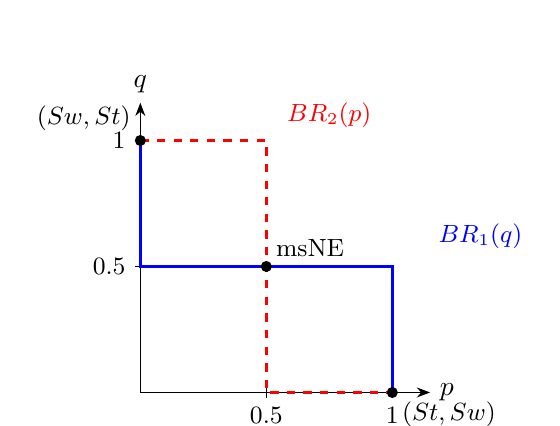
\begin{tikzpicture}[scale=3.2,>=Stealth]
  \draw[->] (0,0) -- (1.15,0) node[right] {$p$};
  \draw[->] (0,0) -- (0,1.15) node[above] {$q$};
  \foreach \t in {0.5,1} {\draw (\t,0.02) -- (\t,-0.02) node[below] {\small $\t$};
                          \draw (0.02,\t) -- (-0.02,\t) node[left] {\small $\t$};}
  % BR_1(q): p = 1 for q < 1/2, any p at q = 1/2, p = 0 for q > 1/2
  \draw[very thick,blue] (1,0) -- (1,0.5) -- (0,0.5) -- (0,1);
  % BR_2(p): q = 1 for p < 1/2, any q at p = 1/2, q = 0 for p > 1/2
  \draw[very thick,red,dashed] (0,1) -- (0.5,1) -- (0.5,0) -- (1,0);
  \fill (1,0) circle (0.022) node[below right] {\small $(St,Sw)$};
  \fill (0,1) circle (0.022) node[above left] {\small $(Sw,St)$};
  \fill (0.5,0.5) circle (0.022) node[above right] {\small msNE};
  \node[blue] at (1.35,0.62) {\small $BR_1(q)$};
  \node[red] at (0.75,1.1) {\small $BR_2(p)$};
\end{tikzpicture}
\end{center}
The two graphs cross three times: at $(p,q) = (1,0)$, i.e.\ $(St,Sw)$; at $(0,1)$, i.e.\
$(Sw,St)$; and at $(\tfrac12,\tfrac12)$, the msNE.

\interp Chicken has the shape of Hawk-Dove (item~7). In the mixed equilibrium each driver goes
straight half of the time, so they crash with probability $\tfrac14$, and each expects $1.5$,
less than the $2$ of mutual swerving and less than the $3$ of the favourable pure equilibrium.
The mix is pinned by the \emph{other} player's indifference, not by one's own payoffs
(slide~50's lesson).

\verify \texttt{check\_A2.py} checks (a)--(c) by brute force, solves both indifference conditions
with sympy ($q^* = p^* = \tfrac12$, payoff $\tfrac32$), and finds on a grid of $(p,q) \in
\{0, \tfrac1{100}, \dots, 1\}^2$ that the mutual best responses are exactly $(1,0)$, $(0,1)$ and
$(\tfrac12,\tfrac12)$. \emph{Comparison with the book's answer} (pp.~87--91): it agrees on all five
parts (no dominated strategies, the same best responses, the two psNE, msNE with $p = q = \tfrac12$,
the same best-response graph, Figs.~3.4--3.6). One typo in the book: on p.~89 the rearranged
indifference condition is printed ``$3 + 3q = q + 2 - 2q \Rightarrow q = 1/2$''; from
$0q + 3(1-q) = 1q + 2(1-q)$ it should read $3 - 3q = q + 2 - 2q$ (as printed, $3 + 3q = 2 - q$ gives
$q = -\tfrac14$). The book's result $q = \tfrac12$ is correct.

\answer{(a) No strictly dominated strategy for either player. (b) $BR_i(St) = Sw$,
$BR_i(Sw) = St$. (c) psNE: $(St, Sw)$ and $(Sw, St)$. (d) msNE: each plays Straight with
probability $\tfrac12$ ($p^* = q^* = \tfrac12$), expected payoff $1.5$ each. (e) $BR_1(q)$: $p = 1$
for $q < \tfrac12$, $p = 0$ for $q > \tfrac12$, any $p$ at $q = \tfrac12$ (symmetric for player~2);
the graphs cross at $(1,0)$, $(0,1)$ and $(\tfrac12,\tfrac12)$.}
\end{exsol}

\begin{exsol}{9}{Tadelis Exercise 5.8}{96--97}{Exam}{L2}
\asked Cournot with $n$ identical firms, $P(Q) = a - Q$, unit cost $c < a$: (a) write the normal
form; (b) find the Nash (Cournot) equilibrium; (c) find the limit of the equilibrium price as
$n \to \infty$ and say what it is.

\method Nash equilibrium with continuous strategies as the crossing of best responses (Tadelis
\S5.2.3, pp.~87--88; Lecture~2, slides~20--27, with the $n$-firm case on slides~26--27).

\solution
\textbf{Book typo.} The statement prints ``$Q = q_i + \cdots + q_n$''. Aggregate production is the
sum over all firms, $Q = q_1 + \cdots + q_n$; the subscript $i$ is a typo for $1$, and the solution
uses $Q = \sum_{j=1}^n q_j$.

\textbf{Notation.} $N = \{1, \dots, n\}$; $q_i \ge 0$ firm $i$'s output; $Q = \sum_j q_j$;
$Q_{-i} = Q - q_i$ the rivals' total; $a > c \ge 0$. The book defines $P(Q) = a - Q$ for $Q \le a$;
for $Q > a$ we take $P = 0$ (Gibbons's convention, p.~15). This only matters off equilibrium:
there a firm earns $-c\,q_i \le 0$.

\textbf{(a) Normal form.} Players $N$; strategies $S_i = [0, \infty)$; payoffs
\[
  u_i(q_i, q_{-i}) = \max\{0,\ a - q_i - Q_{-i}\}\, q_i - c\, q_i . \tag{1}
\]

\textbf{(b) Best response.} Fix $Q_{-i}$. Raising $q_i$ beyond $a - Q_{-i}$ only adds cost, so
consider $q_i \le a - Q_{-i}$, where $u_i = (a - c - Q_{-i} - q_i)\,q_i$ is strictly concave
($\partial^2 u_i/\partial q_i^2 = -2$). The first-order condition is
\[
  a - c - Q_{-i} - 2q_i = 0, \tag{2}
\]
and with the constraint $q_i \ge 0$,
\[
  BR_i(Q_{-i}) = \max\Big\{0,\ \frac{a - c - Q_{-i}}{2}\Big\}. \tag{3}
\]

\textbf{Every firm produces in equilibrium.} Suppose some firm has $q_i^* = 0$. By (3) that
requires $Q_{-i}^* \ge a - c$, so some rival $j$ produces $q_j^* > 0$ and, by (2) for $j$,
$q_j^* = a - c - Q^*$ (because $Q_{-j}^* + 2q_j^* = Q^* + q_j^*$). But $Q^* \ge Q_{-i}^* \ge a - c$
makes $q_j^* \le 0$, a contradiction. So every firm is interior and (2) holds for all $i$.

\textbf{Solving.} Rewrite (2) with $Q_{-i} = Q - q_i$:
\[
  a - c - (Q - q_i) - 2q_i = 0 \;\Longrightarrow\; q_i = a - c - Q . \tag{4}
\]
The right side of (4) is the same for every firm, so all firms produce the same amount, $q_i = q$.
Summing (4) over the $n$ firms:
\[
  Q = n(a - c - Q) \;\Longrightarrow\; (n+1)Q = n(a - c) \;\Longrightarrow\;
  Q^* = \frac{n(a-c)}{n+1}. \tag{5}
\]
Substituting (5) into (4):
\[
  q_i^* = a - c - \frac{n(a-c)}{n+1} = \frac{a-c}{n+1}, \qquad i = 1, \dots, n. \tag{6}
\]
Since $Q^* < a - c < a$, the price is on the linear part of demand:
\[
  P^* = a - Q^* = a - \frac{n(a-c)}{n+1} = \frac{a + nc}{n+1}, \tag{7}
\]
and each firm earns
\[
  u_i^* = (P^* - c)\,q_i^* = \Big(\frac{a + nc}{n+1} - c\Big)\frac{a-c}{n+1}
        = \Big(\frac{a-c}{n+1}\Big)^2 .
\]
The equilibrium is unique: the argument above showed every NE is interior, and (4)--(6) have one
solution. In the slides' notation, $q^m = (a-c)/2$ and (6) reads $q_i^* = 2q^m/(n+1)$; $n = 1$
gives the monopoly output $q^m$ and $n = 2$ gives $\tfrac23 q^m$ (slide~24).

\textbf{(c) Limit.} From (7),
\[
  P^* = \frac{a + nc}{n+1} = c + \frac{a - c}{n+1} \;\xrightarrow[n\to\infty]{}\; c ,
\]
and $Q^* \to a - c = q^{cp}$, the competitive output, with each firm's output and profit going to
zero. This is the familiar perfectly competitive outcome: price equals marginal cost.

\interp The markup $P^* - c = (a-c)/(n+1)$ falls as $1/(n+1)$. Each firm's output lowers the
price for everyone, but a firm counts only the loss on its own units; with more firms its own share
is smaller, so it expands more aggressively and the outcome approaches competition (slide~27).
Contrast with Bertrand (Lecture~2, slides~29--40), where two firms already price at cost.

\verify \texttt{check\_A2.py} solves the $n$ first-order conditions with sympy for
$n = 1, \dots, 6$ and checks (5)--(7) and the profit formula, checks that $P^* - c = (a-c)/(n+1)$
and that the limit is $c$, and confirms numerically ($a = 100$, $c = 10$, $n = 3$) that no
unilateral deviation on a fine grid beats $q_i^* = 22.5$, including the kinked part of demand.
No answer in the book.

\answer{(a) $N = \{1,\dots,n\}$, $S_i = [0,\infty)$,
$u_i = (a - \sum_j q_j)\,q_i - c\,q_i$ (with price $0$ if $\sum_j q_j > a$); the printed
``$Q = q_i + \cdots + q_n$'' should be $q_1 + \cdots + q_n$. (b) Unique NE
$q_i^* = \frac{a-c}{n+1}$, $Q^* = \frac{n(a-c)}{n+1}$, $P^* = \frac{a + nc}{n+1}$, profit
$\big(\frac{a-c}{n+1}\big)^2$. (c) $P^* \to c$: the perfectly competitive price (price $=$
marginal cost).}
\end{exsol}

\begin{exsol}{10}{Tadelis Exercise 6.8}{125}{Exam}{L2}
\asked Three firms decide whether to enter a market; an entrant earns $150/n - 62$ when $n$ firms
enter, a non-entrant $0$. (a) Find all pure-strategy NE; (b) find the symmetric mixed-strategy
NE in which every firm enters with the same probability.

\method Pure NE by checking unilateral deviations (Tadelis Def.~5.1, p.~80); mixed NE by the
principle of indifference (Tadelis Prop.~6.1, p.~108; Lecture~2, slides~44--46), here with three
players.

\solution
\textbf{Notation.} $I = \{1,2,3\}$, $S_i = \{E, O\}$ (enter, stay out). With $n$ entrants an
entrant's payoff is $\pi(n) = 150/n - 62$; staying out pays $0$:
\[
  \pi(1) = 150 - 62 = 88, \qquad \pi(2) = 75 - 62 = 13, \qquad \pi(3) = 50 - 62 = -12 .
\]

\textbf{(a) Pure equilibria.} Classify profiles by the number $n$ of entrants.
\begin{itemize}
  \item $n = 0$: any firm that enters gets $\pi(1) = 88 > 0$. Not NE.
  \item $n = 1$: an outsider that enters gets $\pi(2) = 13 > 0$. Not NE.
  \item $n = 2$: each entrant gets $13 > 0$, so it does not want to leave; the outsider would get
  $\pi(3) = -12 < 0$ by entering, so it stays out. NE.
  \item $n = 3$: each gets $-12 < 0$ and would rather stay out. Not NE.
\end{itemize}
The pure NE are the three profiles in which exactly two firms enter:
$(E,E,O)$, $(E,O,E)$, $(O,E,E)$, each with payoffs $13$ to the entrants and $0$ to the outsider.

\textbf{(b) Symmetric mixed equilibrium.} Let each firm enter with probability $p$. The pure
symmetric profiles are not NE (by (a), $p = 0$ and $p = 1$ fail), so $p \in (0,1)$ and every firm
must be indifferent between $E$ and $O$. Fix firm~$i$. The number of other entrants is $0$, $1$ or
$2$ with probabilities $(1-p)^2$, $2p(1-p)$, $p^2$, so
\[
  u_i(E, p) = (1-p)^2\cdot 88 + 2p(1-p)\cdot 13 + p^2\cdot(-12), \qquad u_i(O, p) = 0. \tag{1}
\]
Expanding the first expression in (1):
\[
  88(1 - 2p + p^2) + 26(p - p^2) - 12p^2 = 88 - 176p + 88p^2 + 26p - 26p^2 - 12p^2
  = 88 - 150p + 50p^2 .
\]
Indifference, $u_i(E,p) = 0$, gives
\[
  50p^2 - 150p + 88 = 0 \;\Longleftrightarrow\; 25p^2 - 75p + 44 = 0,
\]
\[
  p = \frac{75 \pm \sqrt{75^2 - 4\cdot 25\cdot 44}}{2\cdot 25}
    = \frac{75 \pm \sqrt{5625 - 4400}}{50} = \frac{75 \pm 35}{50} \in \Big\{\frac45,\ \frac{11}{5}\Big\}.
\]
Only $p = 4/5$ is a probability. The symmetric mixed NE has each firm entering with probability
$p^* = \tfrac45$, and each firm's expected payoff is $0$ (the payoff of staying out).

Check: at $p = 0.8$, $(0.2)^2\cdot 88 + 2(0.8)(0.2)\cdot 13 + (0.8)^2\cdot(-12)
= 3.52 + 4.16 - 7.68 = 0$.

\interp Entry is a coordination problem over \emph{who} enters: the market supports two firms, not
three. The pure equilibria solve it but need the firms to know who stays out. Without such a
convention, the symmetric equilibrium has each firm entering with probability $0.8$. Then all three
enter with probability $0.8^3 = 0.512$ and lose money, and the expected profit of the industry is
zero: all the rents of the two-firm market are dissipated by miscoordination.

\verify \texttt{check\_A2.py} brute-forces the $2^3$ profiles (pure NE are exactly the three
two-entrant profiles), solves the indifference condition with sympy (roots $\tfrac45$ and
$\tfrac{11}{5}$), and checks that at $p = \tfrac45$ entering and staying out both pay $0$ while
$u_i(E,p)$ is positive for $p < \tfrac45$ and negative for $p \in (\tfrac45, 1]$. No answer in the
book.

\answer{(a) The three profiles with exactly two entrants, $(E,E,O)$, $(E,O,E)$, $(O,E,E)$: each
entrant earns $75 - 62 = 13$, and the outsider would earn $50 - 62 = -12$ by entering. (b) Each
firm enters with probability $p^* = \tfrac45$ (from $50p^2 - 150p + 88 = 0$); expected payoff $0$.}
\end{exsol}

\begin{exsol}{11}{Gibbons Problem 1.6}{49}{Exam}{L2}
\asked Cournot duopoly with $P(Q) = a - Q$ and marginal costs $c_1$, $c_2$: find the NE when
$0 < c_i < a/2$ for both firms, and when $c_1 < c_2 < a$ but $2c_2 > a + c_1$.

\method Cournot equilibrium as the crossing of best responses (Gibbons \S1.2.A, pp.~14--21;
Tadelis \S5.2.3, eq.~(5.2), p.~87; Lecture~2, slides~20--24), now with a corner: a best response
can be $q_i = 0$.

\solution
\textbf{Notation.} $q_i \ge 0$; $P(Q) = a - Q$ for $Q < a$ and $0$ for $Q \ge a$ (the referenced
model, Gibbons p.~15); firm~$i$'s cost $c_i q_i$, $0 \le c_i < a$; $j \ne i$.

\textbf{Best responses.} For $q_i < a - q_j$ the payoff is
\[
  u_i(q_i, q_j) = (a - q_i - q_j - c_i)\,q_i , \tag{1}
\]
strictly concave in $q_i$; for $q_i \ge a - q_j$ the price is zero and $u_i = -c_i q_i \le 0$. The
first-order condition of (1) is $a - c_i - q_j - 2q_i = 0$, so
\[
  BR_i(q_j) = \max\Big\{0,\ \frac{a - c_i - q_j}{2}\Big\}. \tag{2}
\]
The corner $BR_i = 0$ occurs exactly when $q_j \ge a - c_i$: the rival alone already pushes the
price down to $c_i$ or below.

\textbf{Interior candidate.} If both are interior, (2) gives
$2q_1 = a - c_1 - q_2$ and $2q_2 = a - c_2 - q_1$. Substituting $q_2 = (a - c_2 - q_1)/2$ into the
first:
\[
  2q_1 = a - c_1 - \Big(\frac{a - c_2 - q_1}{2}\Big)
  \;\Longrightarrow\; 4q_1 = 2a - 2c_1 - a + c_2 + q_1
  \;\Longrightarrow\; q_1^* = \frac{a - 2c_1 + c_2}{3}, \tag{3}
\]
and symmetrically
\[
  q_2^* = \frac{a - 2c_2 + c_1}{3}. \tag{4}
\]
This is a NE exactly when both (3) and (4) are positive.

\textbf{Case 1: $0 < c_i < a/2$ for $i = 1,2$.} Then $a - 2c_i > 0$, so
$a - 2c_i + c_j > c_j > 0$: (3) and (4) are positive and form a NE. No other NE exists. A corner
NE with $q_2 = 0$ would need $q_1 = BR_1(0) = (a - c_1)/2$ and, by (2), $q_1 \ge a - c_2$, that is,
$(a - c_1)/2 \ge a - c_2 \iff 2c_2 \ge a + c_1$, impossible because $2c_2 < a < a + c_1$. The same
holds for $q_1 = 0$, and $(0,0)$ fails because $BR_i(0) = (a - c_i)/2 > 0$. The unique NE is
\[
  q_1^* = \frac{a - 2c_1 + c_2}{3}, \quad q_2^* = \frac{a - 2c_2 + c_1}{3}, \quad
  Q^* = \frac{2a - c_1 - c_2}{3}, \quad P^* = \frac{a + c_1 + c_2}{3},
\]
with profits $u_i^* = (P^* - c_i)\,q_i^* = (q_i^*)^2$, because
$P^* - c_i = (a + c_1 + c_2 - 3c_i)/3 = (a - 2c_i + c_j)/3 = q_i^*$.

\textbf{Case 2: $c_1 < c_2 < a$ and $2c_2 > a + c_1$.} Now (4) is negative,
$a - 2c_2 + c_1 < 0$, so there is no interior NE. Try firm~1 as a monopolist:
\[
  q_1 = BR_1(0) = \frac{a - c_1}{2}, \qquad q_2 = 0 .
\]
Firm~2's best response to it, by (2):
\[
  BR_2\Big(\frac{a - c_1}{2}\Big) = \max\Big\{0,\ \frac{a - c_2 - \frac{a - c_1}{2}}{2}\Big\}
  = \max\Big\{0,\ \frac{a + c_1 - 2c_2}{4}\Big\} = 0 ,
\]
since $a + c_1 - 2c_2 < 0$. So $\big(\tfrac{a - c_1}{2}, 0\big)$ is a NE. It is the only one: the
other corner, $q_1 = 0$ and $q_2 = (a - c_2)/2$, would need $(a - c_2)/2 \ge a - c_1$, that is,
$2c_1 \ge a + c_2$, but $2c_1 < c_1 + c_2 < a + c_2$; and $(0,0)$ fails as before. At the NE the
price is the monopoly price of firm~1,
\[
  P^* = a - \frac{a - c_1}{2} = \frac{a + c_1}{2} < c_2 ,
\]
so firm~2 cannot sell any unit profitably; firm~1 earns $\big(\frac{a - c_1}{2}\big)^2$.

\interp With similar costs both firms produce, and the cheaper one produces more:
$q_1^* - q_2^* = c_2 - c_1$. When firm~2's cost exceeds firm~1's monopoly price,
$c_2 > (a + c_1)/2$, firm~2 is priced out even though it is not shut out by any rule: firm~1
simply behaves as a monopolist and firm~2's best reply is to stay out. The condition
$2c_2 > a + c_1$ is exactly ``$c_2$ above firm~1's monopoly price''. (Case~1 is sufficient, not
necessary, for the interior NE: (3)--(4) are positive whenever $2c_i < a + c_j$ for both firms,
even if some $c_i \ge a/2$.)

\verify \texttt{check\_A2.py} derives (2)--(4) with sympy, checks $u_i^* = (q_i^*)^2$, and for
random cost pairs in each case finds the NE by iterating the exact best responses (2) and confirms
it equals the formulas above; it also checks on a fine grid that no unilateral deviation pays,
including outputs that push $Q$ above $a$. No answer in the book. (Kumar's unofficial Gibbons
manual, not in \texttt{Livros/}, was not consulted.)

\answer{If $0 < c_i < a/2$: unique NE $q_1^* = \frac{a - 2c_1 + c_2}{3}$,
$q_2^* = \frac{a - 2c_2 + c_1}{3}$, price $\frac{a + c_1 + c_2}{3}$, profits $(q_i^*)^2$.
If $c_1 < c_2 < a$ and $2c_2 > a + c_1$: unique NE $q_1^* = \frac{a - c_1}{2}$, $q_2^* = 0$; firm~1
is a monopolist at price $\frac{a + c_1}{2} < c_2$.}
\end{exsol}

\begin{exsol}{12}{MWG Exercise 8.D.6}{264}{Advanced}{L2}
\asked Prove that every two-player game with two strategies each, with arbitrary payoffs
$u, v, \ell, m, w, x, y, z$ as in the list's matrix, has a mixed-strategy Nash equilibrium.

\method The hint's route: describe each player's strategy by one probability, write the
best-response correspondences, and show they always intersect (MWG \S8.D, Def.~8.D.2 and
Prop.~8.D.1, pp.~250--251, which is the slides' principle of indifference, Lecture~2,
slides~44--46; Tadelis \S6.4, pp.~121--122; Gibbons \S1.3.B, pp.~41--44). Pure equilibria count:
they are degenerate mixed strategies. Nash's theorem (slide~51) gives the result in general; the
point here is a direct proof.

\solution
\textbf{Notation.} $p = \sigma_1(a_1) \in [0,1]$, $q = \sigma_2(b_1) \in [0,1]$. Payoffs:
$u_1(a_1,b_1) = u$, $u_1(a_1,b_2) = \ell$, $u_1(a_2,b_1) = w$, $u_1(a_2,b_2) = y$;
$u_2(a_1,b_1) = v$, $u_2(a_1,b_2) = m$, $u_2(a_2,b_1) = x$, $u_2(a_2,b_2) = z$.

\textbf{Step 1: the payoff gains are affine.} Player~1's gain from $a_1$ over $a_2$ when player~2
plays $q$:
\[
  D_1(q) = \big[qu + (1-q)\ell\big] - \big[qw + (1-q)y\big] = q(u - w) + (1-q)(\ell - y). \tag{1}
\]
Player~2's gain from $b_1$ over $b_2$ when player~1 plays $p$:
\[
  D_2(p) = \big[pv + (1-p)x\big] - \big[pm + (1-p)z\big] = p(v - m) + (1-p)(x - z). \tag{2}
\]
Player~1's expected payoff is $u_1(p,q) = u_1(a_2,q) + p\,D_1(q)$, linear in $p$, so
\[
  BR_1(q) = \begin{cases} \{1\} & D_1(q) > 0,\\ [0,1] & D_1(q) = 0,\\ \{0\} & D_1(q) < 0,\end{cases}
  \qquad
  BR_2(p) = \begin{cases} \{1\} & D_2(p) > 0,\\ [0,1] & D_2(p) = 0,\\ \{0\} & D_2(p) < 0.\end{cases} \tag{3}
\]
$(p^*, q^*)$ is a NE iff $p^* \in BR_1(q^*)$ and $q^* \in BR_2(p^*)$.

\textbf{Step 2: a sign lemma.} An affine function $D$ on $[0,1]$ satisfies exactly one of:
(i) $D(t) \ge 0$ for all $t \in [0,1]$; (ii) $D(t) \le 0$ for all $t$, with $D \not\equiv 0$; or
(iii) $D(0)$ and $D(1)$ are nonzero with opposite signs. In case (iii) $D$ has a unique zero
$t^* = D(0)/(D(0) - D(1)) \in (0,1)$. (If $D(0)$, $D(1)$ are both $\ge 0$ or both $\le 0$, then
$D$, a convex combination of them, keeps that sign on $[0,1]$.)

\textbf{Step 3: the proof, by cases on $D_1$.}

\emph{Case A: $D_1(q) \ge 0$ for all $q$.} Then $p = 1 \in BR_1(q)$ for every $q$ by (3). Let
$\hat q \in BR_2(1)$; it exists because (3) never gives an empty set. Then $1 \in BR_1(\hat q)$
and $\hat q \in BR_2(1)$: $(1, \hat q)$ is a NE.

\emph{Case B: $D_1(q) \le 0$ for all $q$.} Symmetrically, $p = 0$ is a best reply to every $q$,
and $(0, \hat q)$ with $\hat q \in BR_2(0)$ is a NE.

\emph{Case C: $D_1(0)$ and $D_1(1)$ have opposite signs.} Player~1 is indifferent at exactly one
$q^* \in (0,1)$. Solving $D_1(q^*) = 0$ from (1):
\[
  q^* = \frac{y - \ell}{(u - w) + (y - \ell)} . \tag{4}
\]
Now look at $D_2$ and apply the lemma again.
\begin{itemize}
  \item If $D_2(p) \ge 0$ for all $p$: $q = 1$ is a best reply to every $p$; with
  $\hat p \in BR_1(1)$, $(\hat p, 1)$ is a NE.
  \item If $D_2(p) \le 0$ for all $p$: with $\hat p \in BR_1(0)$, $(\hat p, 0)$ is a NE.
  \item If $D_2(0)$, $D_2(1)$ have opposite signs: player~2 is indifferent at
  \[
    p^* = \frac{z - x}{(v - m) + (z - x)} \in (0,1). \tag{5}
  \]
  At $(p^*, q^*)$, $D_1(q^*) = 0$ gives $BR_1(q^*) = [0,1] \ni p^*$, and $D_2(p^*) = 0$ gives
  $BR_2(p^*) = [0,1] \ni q^*$. So $(p^*, q^*)$ is a NE, in strictly mixed strategies.
\end{itemize}
The cases A, B, C exhaust all possibilities by the lemma, and each produces a NE. Hence every game
of this form has a mixed-strategy Nash equilibrium. $\blacksquare$

\interp The argument is the 2$\times$2 version of the fixed-point proof (Tadelis
pp.~121--122): each best-response correspondence is a ``step'' from one side of the unit square to
the other, with a vertical (or horizontal) segment where the player is indifferent, and two such
steps must cross. Mixing is what makes this work: in pure strategies the steps have gaps (Matching
Pennies has no pure NE), and the indifference segment closes the gap. Gibbons's four cases
(p.~42) are the sign patterns of $D_1(0) = \ell - y$ and $D_1(1) = u - w$.

\verify \texttt{check\_A2.py} checks (1), (2), (4) and (5) with sympy, then draws 20{,}000 random
$2\times2$ games (half with integer payoffs in $\{-2,\dots,2\}$, so that ties and constant gains
occur often), runs the case construction above, and confirms with the exact best-response test (3)
that the profile it returns is a NE every time. \emph{Comparison with the MWG solutions manual}
(pp.~8-15--8-16, where the OCR in \texttt{Livros/} prints the number as ``8.0.6''): it splits into
the four strict-dominance cases ($u > w,\ \ell > y$; $u < w,\ \ell < y$; $v > m,\ x > z$;
$v < m,\ x < z$) plus ``all other cases'', where it gives the mixed equilibrium
$\alpha = (y - \ell)/(u + y - \ell - w)$ for player~2 and $\beta = (z - x)/(v + z - x - m)$ for
player~1. These are our (4) and (5); the conclusion agrees. Two remarks on the manual: (i) in
cases~3 and~4 it says ``Player 2 will play his best response'' where it means player~1 (a slip:
the strategies named are $a_1$, $a_2$); (ii) its ``all other cases'' is not complete as written:
if $u = w$ and $\ell = y$ (player~1 indifferent to everything) and player~2 has no strictly
dominant strategy, the formula for $\alpha$ is $0/0$ (any $\alpha$ then works, so an equilibrium
still exists, but the manual's formula does not exhibit it); the same holds for $\beta$ when
$v = m$ and $x = z$. The case split by the sign of $D_1$ above has no such gap.

\answer{With $p = \Pr(a_1)$, $q = \Pr(b_1)$, player~1's gain from $a_1$ is
$D_1(q) = q(u-w) + (1-q)(\ell-y)$ and player~2's gain from $b_1$ is
$D_2(p) = p(v-m) + (1-p)(x-z)$, both affine. If $D_1 \ge 0$ (or $\le 0$) on $[0,1]$, player~1 has a
pure strategy that is always a best reply, and pairing it with player~2's best reply to it is a NE;
the same if $D_2$ keeps a sign. Otherwise both change sign, at
$q^* = \frac{y-\ell}{(u-w)+(y-\ell)}$ and $p^* = \frac{z-x}{(v-m)+(z-x)}$ in $(0,1)$, and
$(p^*, q^*)$ is a NE because each player is indifferent. So a NE always exists.}
\end{exsol}


\part*{Lecture 3 --- Dynamic games and subgame perfection}
\addcontentsline{toc}{part}{Lecture 3 --- Dynamic games and subgame perfection}
\begin{exsol}{13}{Tadelis Exercise 8.8}{171--172}{Foundations}{L3}
\asked Set up the game tree of the entry story (NSG enters or not, then S\&P fights or
accommodates) and find the subgame-perfect equilibrium outcome.

\method Backward induction in a finite game of perfect information (Tadelis \S8.1,
Def.~8.1 and Prop.~8.1, pp.~151--153). With perfect information the subgame-perfect equilibria
are exactly the profiles that survive backward induction (Tadelis \S8.2, p.~158). Same structure
as the entry game of Cabral \S7.2 (\texttt{Notas/L03/L03-06}).

\solution
\textbf{Notation.} Players: NSG (the entrant, E) and S\&P (the incumbent, I). E chooses
$\mathit{In}$ or $\mathit{Out}$; after $\mathit{In}$, I chooses $W$ (price war) or $A$
(accommodate). Payoffs $(u_E, u_I)$ in \$ million of net present value. The entry cost of 2 is
sunk once E enters, so it is subtracted from every payoff that follows $\mathit{In}$:
\begin{align*}
  (u_E,u_I)(\mathit{Out}) &= (0,\ 10),\\
  (u_E,u_I)(\mathit{In},W) &= (1-2,\ 1) = (-1,\ 1),\\
  (u_E,u_I)(\mathit{In},A) &= (4-2,\ 4) = (2,\ 4).
\end{align*}
\begin{center}
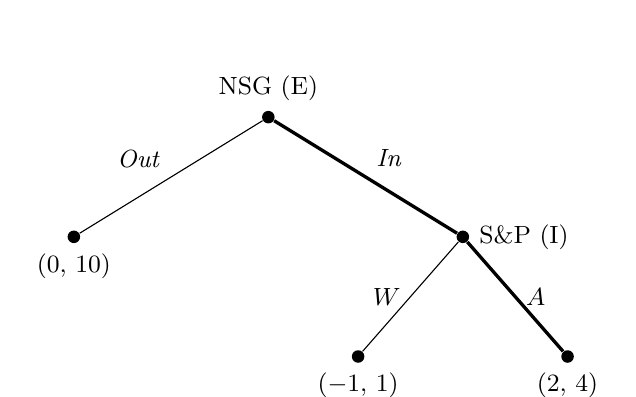
\begin{tikzpicture}[scale=0.95,dot/.style={circle,fill,inner sep=1.6pt},
  every node/.style={font=\small}]
  \node[dot,label=above:{NSG (E)}] (r) at (0,0) {};
  \node[dot,label=below:{$(0,\,10)$}] (o) at (-2.6,-1.6) {};
  \node[dot,label=right:{S\&P (I)}] (i) at (2.6,-1.6) {};
  \node[dot,label=below:{$(-1,\,1)$}] (w) at (1.2,-3.2) {};
  \node[dot,label=below:{$(2,\,4)$}] (a) at (4.0,-3.2) {};
  \draw (r) -- node[above left] {$\mathit{Out}$} (o);
  \draw[very thick] (r) -- node[above right] {$\mathit{In}$} (i);
  \draw (i) -- node[left] {$W$} (w);
  \draw[very thick] (i) -- node[right] {$A$} (a);
\end{tikzpicture}\\[2pt]
{\footnotesize Payoffs $(u_E, u_I)$; thick branches = backward-induction choices.}
\end{center}

\textbf{Step 1: the incumbent's node.} After entry, S\&P compares
\[
  u_I(\mathit{In},A) = 4 > 1 = u_I(\mathit{In},W),
\]
so it accommodates. The price war is not a credible response.

\textbf{Step 2: the entrant's node.} Replacing S\&P's node by its outcome $(2,4)$, NSG compares
\[
  u_E(\mathit{In}) = 2 > 0 = u_E(\mathit{Out}),
\]
so it enters.

\textbf{Step 3: the non-credible Nash equilibrium.} In the normal form (rows: E's strategies;
columns: I's strategies)
\begin{center}
\begin{tabular}{r|c|c|}
\multicolumn{1}{r}{} & \multicolumn{1}{c}{$W$} & \multicolumn{1}{c}{$A$}\\ \cline{2-3}
$\mathit{Out}$ & $0,\ 10$ & $0,\ 10$ \\ \cline{2-3}
$\mathit{In}$ & $-1,\ 1$ & $2,\ 4$ \\ \cline{2-3}
\end{tabular}
\end{center}
there are two pure Nash equilibria, $(\mathit{In},A)$ and $(\mathit{Out},W)$. In
$(\mathit{Out},W)$ the war is never fought, so the threat costs S\&P nothing; it fails
sequential rationality at the node S\&P never reaches (Tadelis Def.~7.8, p.~146; \S8.1).

\interp S\&P's prediction of a price war is cheap talk: once NSG has sunk its \$2 million, a war
gives S\&P 1 instead of 4, and NSG knows it. The incumbent would have to change its own payoffs
(capacity, a contract, a bond) to make the war credible, as in Cabral \S7.2.
The outcome does not depend on how the entry cost is booked: if ``each firm earns \$1 million''
were already net of it, NSG would still enter ($2 > 0$, and even a war would pay $1 > 0$).

\verify \texttt{check\_B\_L03.py} recomputes both backward-induction steps and the two pure
Nash equilibria of the $2\times2$ normal form. Tadelis prints no answer.

\answer{Tree above. Subgame-perfect equilibrium: NSG plays $\mathit{In}$, S\&P plays $A$
(accommodate); outcome: entry and accommodation, payoffs $(2, 4)$ in \$ million (NSG net of the
entry cost). $(\mathit{Out}, W)$ is a Nash equilibrium supported by a non-credible threat.}
\end{exsol}

\begin{exsol}{14}{\MG{} Ch.~4 Exercise 3}{160}{Foundations}{L3}
\asked In the sequential prisoner's dilemma of Fig.~4.9: (a) player~2's best reply to each
move of player~1; (b) player~1's move and the subgame-perfect equilibrium; (c) whether play
differs from the simultaneous version (Ch.~1, Fig.~1.8).

\method Backward induction (Tadelis \S8.1, Prop.~8.1, p.~153). An SPE is written as complete
strategies: player~2's strategy names a reply at \emph{both} of her nodes, including the one off
the path (Tadelis Def.~7.4, p.~139; Gibbons pp.~125--126 on outcome vs.\ equilibrium).

\solution
\textbf{Notation.} $C$ = Confess, $N$ = Not confess. Payoffs $(u_1,u_2)$ from Fig.~4.9:
$(C,C)\mapsto(-5,-5)$, $(C,N)\mapsto(0,-15)$, $(N,C)\mapsto(-15,0)$, $(N,N)\mapsto(-1,-1)$.
Player~2's strategy is a pair $s_2 = (s_2(C), s_2(N))$: her reply after $C$, then after $N$. So
$S_2 = \{CC, CN, NC, NN\}$ and $S_1 = \{C, N\}$.

\textbf{(a) Player 2's best replies.}
\begin{align*}
  \text{after } C:&\quad u_2(C,C) = -5 > -15 = u_2(C,N) \ \Rightarrow\ C;\\
  \text{after } N:&\quad u_2(N,C) = 0 > -1 = u_2(N,N) \ \Rightarrow\ C .
\end{align*}
So $s_2^* = CC$: confess whatever player~1 did.

\textbf{(b) Player 1's move.} Replacing each of player~2's nodes by its outcome,
\[
  u_1(C, s_2^*) = u_1(C,C) = -5 \;>\; -15 = u_1(N,C) = u_1(N, s_2^*),
\]
so player~1 confesses. The SPE is
\[
  (s_1^*, s_2^*) = \bigl(C,\ (C \text{ after } C,\ C \text{ after } N)\bigr) = (C, CC),
\]
with outcome $(C,C)$ and payoffs $(-5,-5)$. In the normal form ($2\times4$) this is also the
only pure Nash equilibrium. If player~1 plays $C$, player~2 must reply $C$ after $C$ ($CC$ or
$CN$), and against $CN$ player~1 would switch to $N$ ($-1 > -5$). If player~1 plays $N$,
player~2 must reply $C$ after $N$ ($CC$ or $NC$), and then $C$ pays player~1 $-5$ or $0$, more
than $-15$.

\textbf{(c) Comparison.} In the simultaneous game (Fig.~1.8) $C$ is strictly dominant for each
prisoner ($-5 > -15$ and $0 > -1$), so the unique Nash equilibrium is $(C,C)$ with $(-5,-5)$. The
sequential version has the same outcome. Seeing player~1's move does not change player~2's
choice, because $C$ is her best reply to each of player~1's moves; player~1 therefore gains
nothing from moving first.

\interp Observing the other's move matters only when the best reply depends on it. Here it does
not: confessing is dominant at both of player~2's nodes, so the sequential game unravels
exactly as the simultaneous one, and the Pareto-better $(N,N)$ is still out of reach. Making a
move observable is a commitment device only when it changes what the follower wants to do (item~17,
Stackelberg).

\verify \texttt{check\_B\_L03.py} computes player~2's replies, player~1's choice, the pure Nash
equilibria of the $2\times4$ normal form (only $(C, CC)$) and of the simultaneous game (only
$(C,C)$). \emph{Comparison with \MG{}'s answer} (pp.~160--162): it agrees on all three parts,
$\text{SPNE} = \{(\text{Confess}, \text{Confess}, \text{Confess})\}$. One wording slip there: the
third component is described as player~2's response ``to player~1 selecting Confess (in
Subgame~3)''; Subgame~3 follows Not Confess, so it is the reply to Not Confess.

\answer{(a) Player~2 confesses after Confess ($-5 > -15$) and after Not confess ($0 > -1$).
(b) Player~1 confesses ($-5 > -15$); SPE $= (C, (C, C))$, outcome $(C,C)$, payoffs $(-5,-5)$.
(c) No difference: the simultaneous game's unique equilibrium is also $(C,C)$, since Confess is
strictly dominant at every node.}
\end{exsol}

\begin{exsol}{15}{Tadelis Exercise 8.10}{172}{Exam}{L3}
\asked Player~1 either plays safe ($S$, payoffs $(3,3)$) or risks ($R$) a simultaneous
$2\times2$ game with player~2. (a) Draw a tree and count its proper subgames; (b) say whether
other trees would do; (c) write the normal form; (d) find all Nash and subgame-perfect equilibria.

\method Extensive form with an information set for the simultaneous stage (Tadelis \S7.1,
Def.~7.2, p.~135); proper subgames (Def.~8.2, pp.~154--155; Tadelis counts the whole game);
strategies as complete plans (Def.~7.4, p.~139); SPE by replacing the subgame with each of its
Nash equilibria (\S8.2, Def.~8.3, p.~157; the voluntary Battle of the Sexes, pp.~154--159, has the
same structure). Mixed equilibria by the indifference principle (Tadelis \S6.1--6.2, pp.~101--114).

\solution
\textbf{Notation.} After $R$, player~1 chooses $C$ or $D$ and player~2 chooses $A$ or $B$
without seeing it. $p = \Pr(C)$, $q = \Pr(A)$ in the subgame.

\textbf{(a) Tree and subgames.}
\begin{center}
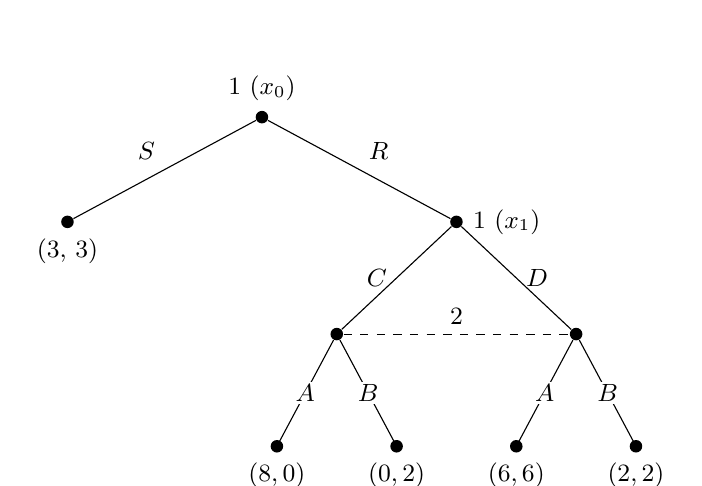
\begin{tikzpicture}[scale=0.95,dot/.style={circle,fill,inner sep=1.6pt},
  every node/.style={font=\small}]
  \node[dot,label=above:{1 ($x_0$)}] (r) at (0,0) {};
  \node[dot,label=below:{$(3,\,3)$}] (s) at (-2.6,-1.4) {};
  \node[dot,label=right:{1 ($x_1$)}] (x1) at (2.6,-1.4) {};
  \node[dot] (c) at (1.0,-2.9) {};
  \node[dot] (d) at (4.2,-2.9) {};
  \draw (r) -- node[above left] {$S$} (s);
  \draw (r) -- node[above right] {$R$} (x1);
  \draw (x1) -- node[left] {$C$} (c);
  \draw (x1) -- node[right] {$D$} (d);
  \draw[dashed] (c) -- node[above] {2} (d);
  \foreach \x/\p/\lab/\pay in {0.2/c/$A$/{$(8,0)$}, 1.8/c/$B$/{$(0,2)$},
                               3.4/d/$A$/{$(6,6)$}, 5.0/d/$B$/{$(2,2)$}} {
    \node[dot,label=below:{\pay}] at (\x,-4.4) {};
    \draw (\p) -- node[fill=white,inner sep=1pt] {\lab} (\x,-4.4);
  }
\end{tikzpicture}
\end{center}
Player~2's two nodes form one information set (dashed). Candidate roots of a proper subgame are
the singleton nodes $x_0$ and $x_1$; player~2's nodes fail (each would cut her information
set). So the game has \textbf{two proper subgames}: the whole game and the simultaneous game that
starts at $x_1$ (one, if, like Gibbons, one does not count the whole game).

\textbf{(b) Other trees.} Yes. (i) In the simultaneous stage, player~2 can be drawn as moving
first at $x_1$ with player~1's two nodes joined in an information set; the strategies, normal
form and subgames are unchanged. (ii) A different tree also represents the story: player~1
picks $S$, $RC$ or $RD$ at the root, and player~2 has one information set over the nodes after
$RC$ and $RD$. Its normal form is the same up to merging $SC$ and $SD$ (it is the
\emph{reduced} normal form), but it has only one proper subgame, the whole game, so subgame
perfection there has no bite: every Nash equilibrium is subgame perfect. The choice of tree matters
for SPE whenever it changes which subgames exist; tree~(i) and the drawing in (a) are the
faithful ones, since $R$ is a real decision taken before the stage game.

\textbf{(c) Normal form.} Player~1 has two information sets, so
$S_1 = \{SC, SD, RC, RD\}$ (first letter at $x_0$, second at $x_1$); $S_2 = \{A, B\}$:
\begin{center}
\begin{tabular}{r|c|c|}
\multicolumn{1}{r}{} & \multicolumn{1}{c}{$A$} & \multicolumn{1}{c}{$B$}\\ \cline{2-3}
$SC$ & $3,\ 3$ & $3,\ 3$ \\ \cline{2-3}
$SD$ & $3,\ 3$ & $3,\ 3$ \\ \cline{2-3}
$RC$ & $8,\ 0$ & $0,\ 2$ \\ \cline{2-3}
$RD$ & $6,\ 6$ & $2,\ 2$ \\ \cline{2-3}
\end{tabular}
\end{center}

\textbf{(d) Equilibria.}

\emph{Step 1: the subgame at $x_1$.} Best replies: $BR_1(A) = C$ ($8 > 6$), $BR_1(B) = D$
($2 > 0$), $BR_2(C) = B$ ($2 > 0$), $BR_2(D) = A$ ($6 > 2$). They cycle, so there is no pure
equilibrium. Player~2 is indifferent when
\begin{equation}
  u_2(A) = 0\cdot p + 6(1-p) \;=\; 2p + 2(1-p) = u_2(B)
  \;\Rightarrow\; 6 - 6p = 2 \;\Rightarrow\; p = \tfrac23 , \label{eq:15p}
\end{equation}
and player~1 is indifferent when
\begin{equation}
  u_1(C) = 8q \;=\; 6q + 2(1-q) = u_1(D)
  \;\Rightarrow\; 8q = 2 + 4q \;\Rightarrow\; q = \tfrac12 . \label{eq:15q}
\end{equation}
The unique equilibrium of the subgame is $(p,q) = (\frac23, \frac12)$, with values
\[
  u_1 = 8\left(\tfrac12\right) = 4, \qquad u_2 = 2 .
\]

\emph{Step 2: subgame-perfect equilibrium.} Replace $x_1$ by $(4,2)$. At $x_0$, $R$ gives $4 > 3$,
so player~1 risks. Since the subgame has a unique equilibrium, the SPE is unique:
\[
  \sigma^{\text{SPE}}:\ \text{player 1 plays } R \text{ and then } C \text{ w.p. } \tfrac23;\
  \text{player 2 plays } A \text{ w.p. } \tfrac12,\qquad \text{payoffs } (4, 2).
\]
In the normal form this is player~1 mixing $\frac23 RC + \frac13 RD$ against $\frac12 A + \frac12 B$.
There is \emph{no} pure-strategy SPE.

\emph{Step 3: all Nash equilibria.} Given $q$, player~1's payoffs are $3$ ($SC$, $SD$), $8q$ ($RC$)
and $2 + 4q$ ($RD$). Player~2's gain from $A$ over $B$ is $0$ against $SC$, $SD$, $-2$ against $RC$
and $+4$ against $RD$.
\begin{itemize}
  \item $q \le \frac14$: $3 \ge 2 + 4q$ and $3 > 8q$, so $S$ is a best reply (strictly, for $q<\frac14$).
  With player~1 on $\{SC,SD\}$ in any mix, player~2 is indifferent, so any such $q$ is a best reply.
  \emph{Nash equilibria.}
  \item $\frac14 < q < \frac12$: $RD$ is the unique best reply ($2+4q > 3$ and $2 + 4q > 8q$);
  then player~2 strictly prefers $A$, i.e.\ $q = 1$. Contradiction.
  \item $q = \frac12$: $RC$ and $RD$ tie at $4 > 3$; player~2 is indifferent only if
  $-2\Pr(RC) + 4\Pr(RD) = 0$, i.e.\ $\frac23 RC + \frac13 RD$. \emph{The SPE above.}
  \item $q > \frac12$: $RC$ is the unique best reply; then player~2 plays $B$, $q = 0$. Contradiction.
\end{itemize}
So the Nash equilibria are
\[
  \bigl\{\,(\text{any mix of } SC, SD;\ q) : 0 \le q \le \tfrac14 \,\bigr\}
  \ \cup\ \bigl\{\,(\tfrac23 RC + \tfrac13 RD;\ q = \tfrac12)\,\bigr\},
\]
and the \emph{pure} Nash equilibria are $(SC, B)$ and $(SD, B)$, both with payoffs $(3,3)$.
None of the first family is subgame perfect: each asks player~2 to play $A$ with probability at
most $\frac14$ in a subgame whose only equilibrium has $q = \frac12$. The ``threat'' to play $B$
deters $R$, but it is not credible once $R$ has been played.

\interp Playing safe is supported only by player~2's threat to play $B$ in the risky game. Once
the risky game starts, both must play its (mixed) equilibrium, which gives player~1 an expected
4, more than the safe 3, so he takes the risk. Player~2 is worse off ($2 < 3$): she would like to
promise $B$, but cannot.

\verify \texttt{check\_B\_L03.py} confirms that the subgame has no pure equilibrium, solves
\eqref{eq:15p}--\eqref{eq:15q} with sympy, finds the pure Nash equilibria $(SC,B)$, $(SD,B)$ of
the $4\times2$ matrix, and scans $q$ over a grid of 241 points plus the critical values
$\frac14, \frac38, \frac12$. A Nash equilibrium exists exactly at $q \in [0, \frac14]$ and
$q = \frac12$, and at $q=\frac12$ the indifference forces $(\frac23, \frac13)$ on $(RC, RD)$.
Tadelis prints no answer.

\answer{(a) Tree above; two proper subgames (the whole game and the simultaneous game after $R$).
(b) Yes: player~2 can be drawn first in the stage game; a tree with root choices
$\{S, RC, RD\}$ gives the same reduced normal form but no proper subgame other than the whole game.
(c) Matrix above, $S_1 = \{SC,SD,RC,RD\}$. (d) Pure Nash: $(SC,B)$, $(SD,B)$; all Nash: player~1
on $S$ (any mix of $SC$, $SD$) with $\Pr(A) \le \frac14$, plus $(\frac23 RC + \frac13 RD,\ \frac12 A
+ \frac12 B)$. Unique SPE: $R$, then $C$ w.p.\ $\frac23$; $A$ w.p.\ $\frac12$; payoffs $(4,2)$. No
pure SPE.}
\end{exsol}

\begin{exsol}{16}{Tadelis Exercise 8.13}{173--174}{Exam}{L3}
\asked A buyer pays a commuting cost $k$ to reach a seller, who then names a take-it-or-leave-it
price. (a) Extensive form and the buyer's reply at the acceptance node; (b) the SPE, its
uniqueness and Pareto optimality; (c) Nash equilibria better for both; (d) whether the seller
would pay $\varepsilon$ to mail a postcard that commits him to a price.

\method Backward induction with a continuum of actions (Tadelis \S8.1 and \S8.3.2, the
Stackelberg logic, pp.~160--163); the ultimatum-game argument for ties (Tadelis Prop.~11.2,
p.~223: the responder must accept at indifference, or the proposer has no best offer). Nash
equilibria sustained by off-path threats (Tadelis Def.~7.8, p.~146). Commitment as a move added
before the game (\texttt{Notas/L03/L03-06}, Cabral \S7.2).

\solution
\textbf{Notation.} Buyer (B) and seller (S). B chooses $G$ (go to the store) or $H$ (stay
home); then S names $p \ge 0$; then B accepts ($Y$) or walks out ($N$). Data: $c > 0$,
$k > 0$, $v > c + k$. Payoffs $(u_B, u_S)$:
\[
  H:\ (0,\ c);\qquad G,p,Y:\ (v - p - k,\ p);\qquad G,p,N:\ (-k,\ c).
\]

\textbf{(a) Extensive form and the buyer's reply.}
\begin{center}
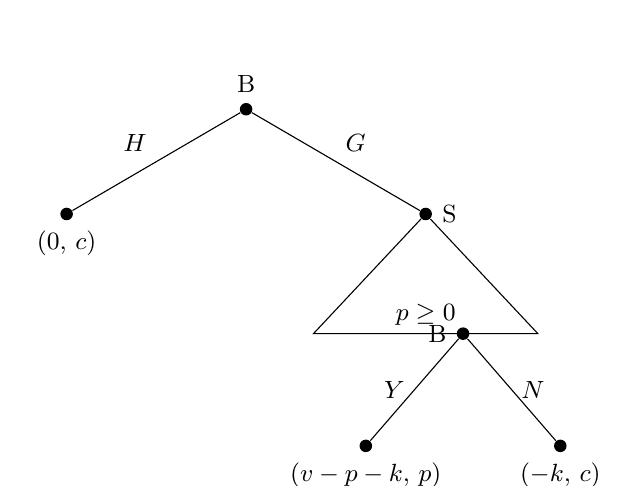
\begin{tikzpicture}[scale=0.95,dot/.style={circle,fill,inner sep=1.6pt},
  every node/.style={font=\small}]
  \node[dot,label=above:{B}] (r) at (0,0) {};
  \node[dot,label=below:{$(0,\,c)$}] (h) at (-2.4,-1.4) {};
  \node[dot,label=right:{S}] (s) at (2.4,-1.4) {};
  \draw (r) -- node[above left] {$H$} (h);
  \draw (r) -- node[above right] {$G$} (s);
  \draw (s) -- (0.9,-3.0) -- (3.9,-3.0) -- (s);
  \node at (2.4,-2.75) {$p \ge 0$};
  \node[dot,label=left:{B}] (b) at (2.9,-3.0) {};
  \node[dot,label=below:{$(v-p-k,\,p)$}] (y) at (1.6,-4.5) {};
  \node[dot,label=below:{$(-k,\,c)$}] (n) at (4.2,-4.5) {};
  \draw (b) -- node[left] {$Y$} (y);
  \draw (b) -- node[right] {$N$} (n);
\end{tikzpicture}\\[2pt]
{\footnotesize The triangle stands for the continuum of prices; one typical price $p$ is drawn.}
\end{center}
At the node after price $p$, the commuting cost is already sunk; it appears in both payoffs. B
accepts if
\[
  v - p - k \;\ge\; -k \iff p \le v .
\]
So the best reply is: accept every $p < v$, reject every $p > v$, and either action at $p = v$.

\textbf{(b) SPE, uniqueness, efficiency.}

\emph{Step 1: the acceptance rule at $p = v$.} Suppose B rejected $p = v$. Then S would get $p$
for every $p < v$ and $c < v$ otherwise, so his payoff approaches $v$ as $p \uparrow v$ but never
reaches it; S would have no best offer, so the profile cannot be an SPE. Hence in every SPE B
accepts if and only if $p \le v$.

\emph{Step 2: the seller.} Given that rule, S's payoff is $p$ for $p \le v$ and $c < v$ for
$p > v$; the unique maximizer is $p^* = v$.

\emph{Step 3: the buyer's commuting decision.} Going yields
\[
  u_B(G) = v - p^* - k = v - (v) - k = -k \;<\; 0 = u_B(H),
\]
so B stays home. Every step had a unique optimum, so the SPE is unique:
\[
  \text{B: } H\text{, and accept iff } p \le v;\qquad \text{S: offer } p = v. \qquad
  \text{Outcome: no trade, payoffs } (0,\ c).
\]
\emph{Not Pareto optimal.} Trade at any price $p \in (c,\ v - k)$ (nonempty since $v > c+k$)
gives $u_B = v - p - k > 0$ and $u_S = p > c$: both strictly better. The lost surplus is
$v - c - k > 0$. This is a hold-up: the commuting cost is sunk when the price is set, so S
extracts all of $v$ and B, anticipating it, never makes the trip.

\textbf{(c) Better Nash equilibria.} Yes. Fix $\hat p \in (c,\ v - k)$ and consider
\[
  \text{B: } G\text{, accept iff } p \le \hat p;\qquad \text{S: offer } \hat p .
\]
\emph{S's best reply:} offers $p \le \hat p$ are accepted and give $p \le \hat p$; offers above are
rejected and give $c < \hat p$. So $\hat p$ is optimal. \emph{B's best reply:} given $\hat p$,
going and accepting gives $v - \hat p - k > 0$, more than staying (0) or going and rejecting
($-k$); B's rule at prices other than $\hat p$ is off the path and does not affect his payoff.
Payoffs $(v - \hat p - k,\ \hat p)$ beat $(0, c)$ for both. It is not subgame perfect: after an
off-path offer $p \in (\hat p, v)$, rejecting gives $-k < v - p - k$, so the threat to walk out
is not credible.

\textbf{(d) The postcard.} Add a first move: S either mails a postcard committing to $\hat p$ (at
cost $\varepsilon$) or does not. Without the postcard the game is the one in (b): payoff $c$ to S.
With it, B buys at $\hat p$ if he goes and $\hat p \le v$, so he goes iff
$v - \hat p - k \ge 0$, i.e.\ $\hat p \le v - k$. By the argument of Step~1, B goes at
indifference. Then S's payoff from the postcard is
\[
  u_S(\hat p) = \begin{cases} \hat p - \varepsilon, & \hat p \le v - k,\\
  c - \varepsilon, & \hat p > v - k, \end{cases}
  \qquad\Rightarrow\qquad \hat p^* = v - k,\quad u_S = v - k - \varepsilon .
\]
Compared with not mailing,
\[
  (v - k - \varepsilon) - c = (v - c - k) - \varepsilon > 0
  \quad\text{since } \varepsilon < v - c - k .
\]
So in the SPE the seller mails the postcard with price $v - k$; B goes and buys; payoffs
$(0,\ v - k - \varepsilon)$. Trade now happens; the total surplus is $v - c - k - \varepsilon$, all
of it to the seller.

\interp The commitment in (c) has to come from the buyer and is not credible; the commitment in
(d) comes from the seller, who limits his own future options, and it is credible because the
coupon binds him. ``Junk mail'' has value even when it contains no information: it is a
commitment not to hold up a customer who has sunk a cost. The seller still captures the whole
surplus; the coupon only removes the inefficiency, the same logic as the bond in the entry game
(Cabral \S7.2).

\verify \texttt{check\_B\_L03.py} uses $c = 2$, $v = 10$, $k = 1$, $\varepsilon = \frac12$ and prices
on a $0.25$ grid: the seller's best offer is $p = 10 = v$ and the buyer stays home; under
``reject at $v$'' the best grid offer is $v - 0.25$ (no maximum on a continuum); thresholds
$\hat p \in \{2.5, 5, 8.5\}$ give Nash equilibria that beat $(0, c)$ for both; with the postcard,
$\hat p^* = 9 = v - k$ and $8.5 > 2$; sympy confirms the gain $(v - c - k) - \varepsilon$. Tadelis
prints no answer.

\answer{(a) Tree above; at the acceptance node the buyer accepts iff $p \le v$ (the sunk $k$ does
not matter). (b) Unique SPE: seller offers $p = v$, buyer accepts iff $p \le v$ and therefore stays
home; payoffs $(0, c)$; not Pareto optimal, since trade at any $p \in (c, v-k)$ helps both. (c) Yes:
buyer goes and accepts only $p \le \hat p$, seller offers $\hat p$, for any $\hat p \in (c, v-k)$;
Nash but not subgame perfect. (d) Yes: the seller mails a coupon at $\hat p = v - k$, the buyer
comes and buys, seller earns $v - k - \varepsilon > c$.}
\end{exsol}

\begin{exsol}{17}{\MG{} Ch.~4 Exercise 12}{185--186}{Exam}{L3}
\asked With $p(Q) = 10 - Q$ and marginal cost 2: (a) the Stackelberg equilibrium with leader~1 and
follower~2; (b) the equilibrium when a third firm moves after firm~2, and how firms~1 and~2's
outputs change.

\method Backward induction with continuous actions: solve the last mover's best reply, substitute
it into the previous mover's profit, repeat (Tadelis \S8.3.2, eqs.~(8.1)--(8.2), pp.~160--161;
Gibbons \S2.1.B, pp.~61--64). The SPE lists each follower's whole reaction function, the outcome
only the quantities (Gibbons pp.~125--126).

\solution
\textbf{Notation.} $q_i \ge 0$ is firm $i$'s output, $Q$ the total; price-cost margin
$p - 2 = 8 - Q$; profit $\pi_i = (8 - Q)\,q_i$.

\textbf{(a) Two firms.}

\emph{Step 1: follower.} Firm~2 maximizes $\pi_2 = (8 - q_1 - q_2)\,q_2$:
\begin{equation}
  \frac{\partial \pi_2}{\partial q_2} = 8 - q_1 - 2q_2 = 0
  \;\Rightarrow\; q_2(q_1) = 4 - \frac{q_1}{2}\quad (q_1 \le 8). \label{eq:17r2}
\end{equation}
\emph{Step 2: leader.} Substituting \eqref{eq:17r2} into $\pi_1$:
\[
  \pi_1 = \Bigl(8 - q_1 - \bigl(4 - \tfrac{q_1}{2}\bigr)\Bigr) q_1
        = \Bigl(4 - \frac{q_1}{2}\Bigr) q_1 ,
  \qquad \frac{d\pi_1}{dq_1} = 4 - q_1 = 0 \;\Rightarrow\; q_1^* = 4 .
\]
\emph{Step 3: outcome.} From \eqref{eq:17r2}, $q_2^* = 4 - \frac{(4)}{2} = 2$; $Q = 6$,
$p = 10 - 6 = 4$, and
\[
  \pi_1 = (4 - 2)(4) = 8, \qquad \pi_2 = (4 - 2)(2) = 4 .
\]
SPE: $\bigl(q_1^* = 4,\ q_2(q_1) = \max\{0, 4 - q_1/2\}\bigr)$.

\textbf{(b) Three firms, moving in the order 1, 2, 3.}

\emph{Step 1: firm 3.} It maximizes $(8 - q_1 - q_2 - q_3)\,q_3$:
\begin{equation}
  8 - q_1 - q_2 - 2q_3 = 0 \;\Rightarrow\; q_3(q_1,q_2) = 4 - \frac{q_1 + q_2}{2}. \label{eq:17r3}
\end{equation}
\emph{Step 2: firm 2.} Substituting \eqref{eq:17r3} into $\pi_2$:
\[
  \pi_2 = \Bigl(8 - q_1 - q_2 - \bigl(4 - \tfrac{q_1+q_2}{2}\bigr)\Bigr) q_2
        = \Bigl(4 - \frac{q_1 + q_2}{2}\Bigr) q_2 ,
\]
\begin{equation}
  \frac{\partial \pi_2}{\partial q_2} = 4 - \frac{q_1}{2} - q_2 = 0
  \;\Rightarrow\; q_2(q_1) = 4 - \frac{q_1}{2}. \label{eq:17r2b}
\end{equation}
Substituting \eqref{eq:17r2b} into \eqref{eq:17r3}:
\[
  q_3(q_1) = 4 - \frac{q_1 + \bigl(4 - \frac{q_1}{2}\bigr)}{2} = 2 - \frac{q_1}{4}.
\]
\emph{Step 3: firm 1.} Substituting both:
\[
  \pi_1 = \Bigl(8 - q_1 - \bigl(4 - \tfrac{q_1}{2}\bigr) - \bigl(2 - \tfrac{q_1}{4}\bigr)\Bigr) q_1
        = \Bigl(2 - \frac{q_1}{4}\Bigr) q_1 ,
  \qquad \frac{d\pi_1}{dq_1} = 2 - \frac{q_1}{2} = 0 \;\Rightarrow\; q_1^* = 4 .
\]
\emph{Step 4: outcome.} $q_2^* = 4 - \frac{(4)}{2} = 2$, $q_3^* = 2 - \frac{(4)}{4} = 1$;
$Q = 7$, $p = 3$, margin $1$:
\[
  \pi_1 = 4,\qquad \pi_2 = 2,\qquad \pi_3 = 1 .
\]
\emph{Comparison.} Firms~1 and~2 produce exactly what they produced in (a), 4 and 2; firm~3 adds 1.
Total output rises from 6 to 7, the price falls from 4 to 3, and the profits of firms~1 and~2 halve
(8 to 4, and 4 to 2).

\interp Why do the outputs not move? Firm~3 absorbs half of any change in $q_1 + q_2$
(slope $-\frac12$ in \eqref{eq:17r3}). After substituting it, firm~2's residual margin is
$4 - \frac{q_1 + q_2}{2}$, half of the margin it faced in (a): the same problem scaled by $\frac12$,
so the same maximizer. The same scaling repeats upstream, which gives the pattern
$q_k = (a - c)/2^k$ for the $k$-th mover with demand $a - Q$ and marginal cost $c$ (here
$a - c = 8$: $4, 2, 1$). The leader always produces the
monopoly output $(a-c)/2 = 4$. Entry at the end of the chain does not change earlier outputs, but
it lowers their profits through the price.

\verify \texttt{check\_B\_L03.py} redoes every first-order condition with sympy (reaction functions,
$q^* = (4,2)$ and $(4,2,1)$, prices 4 and 3, profits $(8,4)$ and $(4,2,1)$, concavity of the
leader's problem) and repeats both games numerically with the leader on a $0.01$ grid. \emph{Comparison
with \MG{}'s answer} (pp.~186--189): same quantities, $(4,2)$ and $(4,2,1)$, and the same conclusion
that firms~1 and~2 do not change output. The book reports no prices or profits. Minor slips in its
text: the interior condition of firm~2's first-order condition is written ``if $q_1 > 0$'' where
$q_2 > 0$ is meant, both in (a) and in (b).

\answer{(a) $q_1 = 4$, $q_2 = 4 - q_1/2 = 2$; $p = 4$; $\pi = (8, 4)$. (b) $q_1 = 4$,
$q_2 = 4 - q_1/2 = 2$, $q_3 = 4 - (q_1+q_2)/2 = 1$; $p = 3$; $\pi = (4,2,1)$. Firms~1 and~2's outputs
are unchanged by firm~3's entry; their profits halve because the price falls.}
\end{exsol}

\begin{exsol}{18}{Gibbons Problem 2.1}{130}{Advanced}{L3}
\asked Prove Becker's Rotten Kid theorem: when a child's action $A$ produces incomes
$I_C(A)$, $I_P(A)$ and an altruistic parent then chooses a bequest $B$, the backwards-induction
outcome has the child choosing the $A$ that maximizes $I_C(A) + I_P(A)$.

\method Backward induction in a two-stage game with continuous actions (Gibbons \S2.1.A,
pp.~57--61; Tadelis \S8.3.2): solve the parent's problem for every pair of incomes, then the
child's problem given the parent's reply. The key step is that the parent's reply depends on the
incomes only through their sum, and raises the child's consumption when the sum rises.

\solution
\textbf{Notation and assumptions.} $A \ge 0$ the child's action; $I_C, I_P$ strictly concave with
maximizers $A_C, A_P > 0$; $B \in \mathbb{R}$ the bequest; $U, V$ increasing and strictly concave;
$k > 0$. Write $Y = I_C + I_P$ (family income) and $x = I_C + B$ (the child's consumption), so the
parent consumes $I_P - B = Y - x$. As is standard for this problem, $U$ and $V$ are
differentiable and the parent's problem has a solution.

\textbf{Step 1: the parent's problem depends only on $Y$.} Given $(I_C, I_P)$ the parent solves
\[
  \max_{B \in \mathbb{R}}\ V(I_P - B) + k\,U(I_C + B).
\]
Because $B$ is unrestricted in sign, choosing $B$ is the same as choosing $x = I_C + B \in \mathbb{R}$,
and the problem becomes
\begin{equation}
  \max_{x \in \mathbb{R}}\ W(x; Y) = V(Y - x) + k\,U(x). \label{eq:18W}
\end{equation}
$W$ is strictly concave in $x$ (a sum of strictly concave functions), so the maximizer $x^*(Y)$ is
unique and satisfies the first-order condition
\begin{equation}
  V'(Y - x^*) = k\,U'(x^*). \label{eq:18foc}
\end{equation}
The bequest is $B^*(I_C, I_P) = x^*(I_C + I_P) - I_C$: it depends on both incomes, but the child's
consumption depends only on their sum.

\textbf{Step 2: $x^*$ is strictly increasing in $Y$.} Take $Y' > Y$ and suppose
$x' = x^*(Y') \le x = x^*(Y)$. Then $Y' - x' > Y - x$. Strict concavity makes $V'$ strictly
decreasing and $U'$ decreasing, so
\[
  V'(Y' - x') < V'(Y - x) \qquad\text{and}\qquad k\,U'(x') \ge k\,U'(x).
\]
Applying \eqref{eq:18foc} at $Y$ and at $Y'$:
\[
  V'(Y' - x') = k\,U'(x') \;\ge\; k\,U'(x) = V'(Y - x) \;>\; V'(Y' - x'),
\]
a contradiction. Hence $x^*(Y') > x^*(Y)$. (With $U, V$ twice differentiable,
$dx^*/dY = V''/(V'' + kU'') \in (0,1)$: the parent passes part, not all, of an income gain to the
child.)

\textbf{Step 3: the child's problem.} Anticipating $B^*$, the child chooses $A \ge 0$ to maximize
\[
  U\bigl(I_C(A) + B^*(I_C(A), I_P(A))\bigr) = U\bigl(x^*(I_C(A) + I_P(A))\bigr) = U\bigl(x^*(Y(A))\bigr).
\]
$U \circ x^*$ is strictly increasing (Steps~1--2 and $U$ increasing), so $A$ maximizes the child's
payoff if and only if it maximizes $Y(A) = I_C(A) + I_P(A)$.

\textbf{Step 4: the maximizer exists and is unique.} $Y$ is strictly concave. For
$A < \min\{A_C, A_P\}$ both incomes are increasing, and for $A > \max\{A_C, A_P\}$ both are
decreasing, so $Y$ attains its maximum on the compact interval $[\min\{A_C,A_P\}, \max\{A_C,A_P\}]
\subset (0, \infty)$, at a unique point $A^*$. The backwards-induction outcome is
\[
  \bigl(A^*,\ B^*(I_C(A^*), I_P(A^*))\bigr), \qquad A^* = \arg\max_{A \ge 0}\ [\,I_C(A) + I_P(A)\,].
  \qquad\square
\]

\interp The child is selfish but faces a parent who ``taxes'' any loss of family income: if the
child raised $I_C$ at a larger cost to $I_P$, the parent, who cares about the split, would cut the
bequest by more than the child gained. Altruism on one side, plus the parent's last move, aligns the
first mover's incentives with joint surplus. The theorem needs the parent to move last with an
unrestricted transfer: if $B \ge 0$ were imposed and binding, or if the child moved after the
bequest, Step~1 would fail. Note that the child does \emph{not} pick $A_C$; it is between $A_C$ and
$A_P$.

\verify \texttt{check\_B\_L03.py} checks the sign of $dx^*/dY$ for several values of
$(V'', U'', k)$, and solves an example numerically: $U = V = -e^{-x}$, $k = 2$,
$I_C = 4A - A^2$ ($A_C = 2$), $I_P = 10A - A^2$ ($A_P = 5$). For each $A$ on a $0.05$ grid it finds
the parent's best bequest on a fine grid; the child's best action is $A = 3.5$, the maximizer of
$I_C + I_P = 14A - 2A^2$, not $A_C = 2$. The child's consumption matches the closed form
$x^* = (Y + \ln k)/2$, which is increasing in $Y$. Gibbons prints no answer.

\answer{The parent's best bequest gives the child consumption $x^*(I_C + I_P)$ that solves
$V'(Y - x) = kU'(x)$; it depends only on family income $Y$ and is strictly increasing in it. So the
child's payoff $U(x^*(Y(A)))$ is a strictly increasing function of $Y(A)$, and the child chooses
$A^* = \arg\max_A [I_C(A) + I_P(A)]$, which exists and is unique by strict concavity.}
\end{exsol}


\part*{Lecture 4 --- Multistage games and bargaining}
\addcontentsline{toc}{part}{Lecture 4 --- Multistage games and bargaining}
\begin{exsol}{19}{Tadelis Exercise 9.1}{186--187}{Foundations}{L4}
\asked The $3\times3$ game is played twice with the first-period outcome observed. (a) All
pure-strategy SPE with $\delta = 1$, with history-contingent strategies; (b) for each, the smallest
$\delta$ that supports it.

\method Multistage games (Tadelis \S9.1--9.4, pp.~175--184): period-2 play must be a stage Nash
equilibrium after every history (Prop.~9.2, p.~181), and a non-equilibrium first-period profile
can be supported only with a carrot (a good stage equilibrium on the path) and a stick (a bad one
after a deviation), when $\delta \ge \delta^* = g/(c - s)$ (\texttt{Notas/L04/L04-02}). Deviations
are checked one stage at a time (one-stage deviation principle, Thm.~9.1, p.~185).

\solution
\textbf{Notation.} $v_i = u_i(a^1) + \delta\, u_i(a^2)$, where $a^t$ is the period-$t$ action
profile. A pure strategy for player~$i$ is a period-1 action and a map from the nine possible
period-1 outcomes to a period-2 action. $g_i(a)$ is player~$i$'s best one-shot gain from deviating
from $a$:
\[
  g_1(a) = \max_{r} u_1(r, a_2) - u_1(a), \qquad g_2(a) = \max_{c} u_2(a_1, c) - u_2(a).
\]

\textbf{Step 1: stage equilibria.} Best replies of player~1: to $L$, $B$ (13); to $C$, $M$ (5);
to $R$, $B$ (1). Of player~2: to $T$, $R$ (13); to $M$, $C$ (5); to $B$, $R$ (1). The mutual best
replies are
\[
  (M, C)\ \text{with } (5,5) \quad\text{(the carrot)}, \qquad (B, R)\ \text{with } (1,1)
  \quad\text{(the stick)} .
\]
Each player gets 5 in the carrot and 1 in the stick, so the largest punishment is $c - s = 5 - 1 = 4$.

\textbf{Step 2: which first-period profiles can be supported.} Period-2 play is $(M,C)$ or
$(B,R)$ after every history. A first-period profile $a$ is supportable if and only if each player's
gain is at most what the threat can take away:
\begin{equation}
  g_i(a) \;\le\; \delta\,(5 - 1) = 4\delta, \qquad i = 1, 2, \label{eq:19ic}
\end{equation}
using $(M,C)$ after $a$ and $(B,R)$ after any deviation. No continuation can do better, since 5 is
the most and 1 the least a player can get in period~2. For a stage equilibrium $a$, $g_i(a) = 0$
and any continuation works. The gains are:
\begin{center}
\small
\begin{tabular}{lccccc}
\toprule
$a$ & $u(a)$ & $g_1(a)$ & $g_2(a)$ & supportable ($\delta=1$)? & $\delta^* = \max_i g_i/4$\\
\midrule
$(T,L)$ & $(10,10)$ & $13-10=3$ & $13-10=3$ & yes & $3/4$ \\
$(T,C)$ & $(2,12)$ & $5-2=3$ & $13-12=1$ & yes & $3/4$ \\
$(T,R)$ & $(0,13)$ & $1-0=1$ & $0$ & yes & $1/4$ \\
$(M,L)$ & $(12,2)$ & $13-12=1$ & $5-2=3$ & yes & $3/4$ \\
$(M,C)$ & $(5,5)$ & $0$ & $0$ & yes & $0$ \\
$(M,R)$ & $(0,0)$ & $1-0=1$ & $5-0=5$ & no & -- \\
$(B,L)$ & $(13,0)$ & $0$ & $1-0=1$ & yes & $1/4$ \\
$(B,C)$ & $(0,0)$ & $5-0=5$ & $1-0=1$ & no & -- \\
$(B,R)$ & $(1,1)$ & $0$ & $0$ & yes & $0$ \\
\bottomrule
\end{tabular}
\end{center}

\textbf{(a) The pure SPE with $\delta = 1$.} The SPE \emph{paths} are nine:
\begin{itemize}
  \item the four sequences of stage equilibria, played regardless of history (Prop.~9.1, p.~180):
  $(M,C)$ then $(M,C)$; $(M,C)$ then $(B,R)$; $(B,R)$ then $(M,C)$; $(B,R)$ then $(B,R)$;
  \item the five carrot-and-stick paths: $a$ then $(M,C)$, for $a \in \{(T,L), (T,C), (T,R),
  (M,L), (B,L)\}$.
\end{itemize}
For a carrot-and-stick path the strategies are, for $\hat a = (\hat a_1, \hat a_2)$ one of those five:
\begin{align*}
  s_1&:\ \text{play } \hat a_1;\ \text{in period 2 play } M \text{ if } \hat a \text{ was played, } B
  \text{ otherwise};\\
  s_2&:\ \text{play } \hat a_2;\ \text{in period 2 play } C \text{ if } \hat a \text{ was played, } R
  \text{ otherwise}.
\end{align*}
For example, for $(T,L)$: on the path each gets $10 + 5 = 15$; player~1's best deviation ($B$) gives
$13 + 1 = 14$, player~2's ($R$) gives $13 + 1 = 14$. In period~2 both play a stage equilibrium after
every history, so no deviation pays there. $(M,R)$ and $(B,C)$ cannot be supported: a gain of 5
exceeds the largest punishment 4.

These strategies are not the only ones. Any assignment of $(M,C)$ or $(B,R)$ to the nine period-1 outcomes
that satisfies \eqref{eq:19ic} for the deviations that would be profitable also works (e.g.\ for
$(T,R)$ only player~1's deviation to $B$ must be punished). Counting every such map,
\texttt{check\_B\_L04.py} finds 992 pure SPE strategy profiles at $\delta = 1$, all with one of the
nine paths above.

\textbf{(b) The smallest discount factor.} From \eqref{eq:19ic},
$\delta^*(a) = \max_i g_i(a)/4$ (last column): $\frac34$ for $(T,L)$, $(T,C)$, $(M,L)$;
$\frac14$ for $(T,R)$, $(B,L)$; and any $\delta \ge 0$ for the four sequences of stage equilibria.
For $(T,L)$: $10 + 5\delta \ge 13 + \delta \iff \delta \ge \frac34$.

\interp Two stage equilibria with different payoffs give the second period a carrot and a stick,
and that lets the players reach $(T,L)$, which pays $(10,10)$, twice the $(5,5)$ of the good stage
equilibrium, in the first period. Profiles with a gain above $4$ cannot be enforced by a single
future period, however patient the players are.

\verify \texttt{check\_B\_L04.py} finds the two stage equilibria, enumerates all $9 \times 2^9$
combinations of first-period profile and continuation map at $\delta = 1$ (992 SPE, 9 paths;
$(M,R)$ and $(B,C)$ excluded), and checks every threshold: each path is an SPE at $\delta^*$, and
no continuation map at all supports it at $\delta^* - 0.001$. Tadelis prints no answer.

\answer{Stage equilibria: $(M,C)$ $(5,5)$ and $(B,R)$ $(1,1)$. (a) Pure SPE paths with $\delta=1$:
the four sequences of stage equilibria, and $a$ then $(M,C)$ for $a \in \{(T,L),(T,C),(T,R),
(M,L),(B,L)\}$, supported by ``play $(M,C)$ after $a$, $(B,R)$ after any other outcome''.
$(M,R)$ and $(B,C)$ cannot be supported. (b) $\delta^* = \frac34$ for $(T,L)$, $(T,C)$, $(M,L)$;
$\frac14$ for $(T,R)$, $(B,L)$; $0$ for the sequences of stage equilibria.}
\end{exsol}

\begin{exsol}{20}{Gibbons Problem 2.6}{133}{Foundations}{L4}
\asked Firm~1 chooses $q_1$; firms~2 and~3 observe it and choose $q_2, q_3$ simultaneously;
demand $P = a - Q$, marginal cost $c$. Find the subgame-perfect outcome.

\method Two-stage game of complete but imperfect information (Gibbons \S2.2.A, pp.~71--73): for each
$q_1$ solve the second-stage simultaneous game for its Nash equilibrium, then let firm~1 optimize
against it. The second stage is a Cournot duopoly on the residual demand (Gibbons \S1.2.A); the
first stage is Stackelberg logic (Gibbons \S2.1.B; Tadelis \S8.3.2).

\solution
\textbf{Notation.} $a > c \ge 0$; $q_i \ge 0$; profit $\pi_i = (a - Q - c)\,q_i$ with
$Q = q_1 + q_2 + q_3$.

\textbf{Step 1: second stage, given $q_1 < a - c$.} Firm~2's and firm~3's first-order conditions:
\begin{align}
  \frac{\partial\pi_2}{\partial q_2} &= a - c - q_1 - 2q_2 - q_3 = 0, \label{eq:20a}\\
  \frac{\partial\pi_3}{\partial q_3} &= a - c - q_1 - q_2 - 2q_3 = 0. \label{eq:20b}
\end{align}
Subtracting \eqref{eq:20b} from \eqref{eq:20a} gives $q_3 - q_2 = 0$, so $q_2 = q_3$. Substituting
$q_3 = q_2$ into \eqref{eq:20a}:
\[
  a - c - q_1 - 2q_2 - (q_2) = 0 \;\Rightarrow\; q_2(q_1) = q_3(q_1) = \frac{a - c - q_1}{3}.
\]
This is the Cournot duopoly with demand intercept $a - q_1$; its equilibrium is unique. If
$q_1 \ge a - c$, both followers produce $0$.

\textbf{Step 2: first stage.} Substituting the followers' outputs, for $q_1 < a - c$,
\[
  \pi_1 = \Bigl(a - q_1 - 2\cdot\frac{a - c - q_1}{3} - c\Bigr) q_1
        = \frac{a - c - q_1}{3}\, q_1 ,
\]
a strictly concave function with
\[
  \frac{d\pi_1}{dq_1} = \frac{a - c - 2q_1}{3} = 0 \;\Rightarrow\; q_1^* = \frac{a - c}{2}.
\]
For $q_1 \ge a - c$ the price is at most $c$, so $\pi_1 \le 0$; the interior choice is the global one.

\textbf{Step 3: outcome.}
\[
  q_2^* = q_3^* = \frac{a - c - \frac{a-c}{2}}{3} = \frac{a - c}{6}, \qquad
  Q^* = \frac{a-c}{2} + 2\cdot\frac{a-c}{6} = \frac{5(a - c)}{6},
\]
\[
  P^* = a - \frac{5(a-c)}{6} = \frac{a + 5c}{6},
\]
\[
  \pi_1^* = \frac{a - c}{6}\cdot\frac{a - c}{2} = \frac{(a-c)^2}{12}, \qquad
  \pi_2^* = \pi_3^* = \frac{a-c}{6}\cdot\frac{a-c}{6} = \frac{(a-c)^2}{36}.
\]
The subgame-perfect outcome is $\bigl(q_1^*, q_2^*, q_3^*\bigr) = \bigl(\frac{a-c}{2},
\frac{a-c}{6}, \frac{a-c}{6}\bigr)$. The SPE itself lists the followers' strategies
$q_2(q_1) = q_3(q_1) = \max\{0, (a - c - q_1)/3\}$.

\interp The leader again chooses the monopoly output $(a-c)/2$, as in the two-firm Stackelberg game
(Gibbons p.~63) and in item~17: with linear demand, the followers' joint reply has slope
$-\frac23$, and the leader's residual margin $(a - c - q_1)/3$ is a scaled copy of the monopoly
margin. Compared with simultaneous three-firm Cournot (each $(a-c)/4$, $Q = \frac34(a-c)$), the
leader produces more and earns more ($\frac{(a-c)^2}{12} > \frac{(a-c)^2}{16}$), the followers less,
and total output is higher.

\verify \texttt{check\_B\_L04.py} solves \eqref{eq:20a}--\eqref{eq:20b} and firm~1's problem with
sympy and checks $Q^*$, $P^*$ and both profits; it also solves the case $a = 13$, $c = 1$ with
the leader on a grid of step $0.05$: $q_1 = 6$, $q_2 = q_3 = 2$. Gibbons prints no answer.

\answer{$q_1^* = \frac{a-c}{2}$, $q_2^* = q_3^* = \frac{a-c}{6}$ (followers' rule
$q_j(q_1) = \max\{0, \frac{a-c-q_1}{3}\}$); $P^* = \frac{a+5c}{6}$; profits
$\frac{(a-c)^2}{12}$ for firm~1 and $\frac{(a-c)^2}{36}$ for each follower.}
\end{exsol}

\begin{exsol}{21}{Tadelis Exercise 9.4}{188}{Exam}{L4}
\asked A Cournot stage ($p = 100 - q$, zero cost) is followed by an ``access'' game with
equilibria $(O,o)$ and $(N,n)$. (a) The Cournot equilibrium, the access game's pure equilibria and
all pure SPE when $\delta = 0$; (b) an SPE with monopoly output split equally when $\delta = 1$;
(c) the lowest $\delta$ for it; (d) whether it survives at $\delta = 0.4$, and if not the best
symmetric profits.

\method Multistage games with a carrot and a stick in the last stage (Tadelis \S9.4,
pp.~180--184; threshold $\delta^* = g/(c - s)$, \texttt{Notas/L04/L04-02}); Cournot best replies
(Tadelis \S5.2.3, pp.~87--88). Payoffs $v_i = \pi_i(q_1, q_2) + \delta\,u_i(\text{access})$.

\solution
\textbf{(a) Stage games and $\delta = 0$.}

\emph{Cournot.} Firm $i$ maximizes $(100 - q_i - q_j)\,q_i$:
\begin{equation}
  100 - 2q_i - q_j = 0 \;\Rightarrow\; q_i = BR_i(q_j) = \frac{100 - q_j}{2}. \label{eq:21br}
\end{equation}
By symmetry $q_i = q_j = q$, so $q = \frac{100 - q}{2}$, i.e.\ $q^C = \frac{100}{3}$, price
$\frac{100}{3}$, and $\pi^C = \bigl(\frac{100}{3}\bigr)^2 = \frac{10000}{9} \approx 1111.1$ each.

\emph{Access game.} Payoffs (player~1 rows):
\begin{center}
\begin{tabular}{r|c|c|}
\multicolumn{1}{r}{} & \multicolumn{1}{c}{$o$} & \multicolumn{1}{c}{$n$}\\ \cline{2-3}
$O$ & $2500,\ 2500$ & $-10,\ 0$ \\ \cline{2-3}
$N$ & $0,\ -10$ & $0,\ 0$ \\ \cline{2-3}
\end{tabular}
\end{center}
$O$ is the best reply to $o$ ($2500 > 0$) and $N$ the best reply to $n$ ($0 > -10$); symmetrically
for player~2. Pure equilibria: $(O,o)$ with $(2500, 2500)$ and $(N,n)$ with $(0,0)$.

\emph{SPE with $\delta = 0$.} Stage-2 payoffs carry weight $0$, so continuation play cannot reward or
punish anything, and stage~1 must be the Cournot equilibrium. The pure SPE are
\[
  s_i:\ q_i = \tfrac{100}{3};\ \text{in stage 2, after each } (q_1, q_2),\ \text{play the action
  of } e(q_1, q_2),
\]
where $e$ is \emph{any} map from $\mathbb{R}_+^2$ to $\{(O,o), (N,n)\}$ (e.g.\ always $(O,o)$).
There is a continuum of them, all with first-stage outcome $(\frac{100}{3}, \frac{100}{3})$.
Strictly, with $\delta = 0$ the stage-2 actions do not affect any payoff, so every stage-2 profile
is an equilibrium of those subgames; the answer above uses the standard reading that stage-2
actions are judged by stage-2 payoffs (the limit $\delta \to 0^+$).

\textbf{(b) Monopoly split with $\delta = 1$.} Joint profit $(100 - Q)Q$ is maximized at $Q = 50$;
each firm produces $25$ and earns
\[
  \pi^M = 25\,(100 - 50) = 1250 .
\]
Strategies (for both firms):
\[
  s_i:\ q_i = 25;\ \text{in stage 2, open } (O / o) \text{ if } (q_1,q_2) = (25,25),\ \text{keep
  closed } (N / n) \text{ otherwise}.
\]
\emph{Stage 2.} After every history the prescribed profile is an equilibrium of the access game.
\emph{Stage 1.} The best deviation against $q_j = 25$ is, by \eqref{eq:21br},
$q_i = \frac{100 - 25}{2} = 37.5$, with price $100 - 62.5 = 37.5$ and
\[
  \pi^D = 37.5 \times 37.5 = 1406.25 .
\]
Staying gives $1250 + \delta\,(2500)$; deviating gives $1406.25 + \delta\,(0)$. With $\delta = 1$:
$3750 \ge 1406.25$. It is an SPE.

\textbf{(c) Lowest $\delta$.}
\begin{equation}
  1250 + 2500\,\delta \;\ge\; 1406.25 \iff \delta \;\ge\; \delta^* = \frac{156.25}{2500} = \frac{1}{16} = 0.0625 .
  \label{eq:21d}
\end{equation}
In the carrot-and-stick form: $g = 156.25$, $c - s = 2500 - 0$.

\textbf{(d) $\delta = 0.4$.} Since $0.4 > \frac1{16}$, condition \eqref{eq:21d} holds:
$1250 + 0.4\,(2500) = 2250 \ge 1406.25$. The monopoly split \emph{is} supported, with the same
strategies as in (b), and each firm earns $2250$ in discounted total. The ``if not'' branch does not
arise with these numbers.

For completeness, when $\delta < \frac1{16}$: with symmetric output $q$ and the same threat, the
deviation gain is
\[
  g(q) = \Bigl(\frac{100 - q}{2}\Bigr)^2 - q\,(100 - 2q) = \frac94\Bigl(\frac{100}{3} - q\Bigr)^2 ,
\]
and $g(q) \le 2500\,\delta$ holds iff $q \ge \frac{100}{3}(1 - \sqrt{\delta})$. The best symmetric
equilibrium uses $q = \max\{25,\ \frac{100}{3}(1 - \sqrt\delta)\}$; e.g.\ at $\delta = 0.04$,
$q = \frac{80}{3}$ and stage-1 profit $\frac{11200}{9} \approx 1244.4$ each.

\interp The second stage is worth far more ($2500$) than the one-shot gain from cheating on the
cartel ($156.25$), so even very impatient firms ($\delta \ge 0.0625$) can collude in stage~1. The
threat is credible because $(N,n)$ is itself an equilibrium: once someone cheats, neither firm
wants to be the only one to open. A future coordination game with a good and a bad equilibrium is
an effective enforcement device, which is the multistage logic of Tadelis \S9.4.

\verify \texttt{check\_B\_L04.py} recomputes the Cournot equilibrium ($\frac{100}{3}$,
$\frac{10000}{9}$), the two pure equilibria of the access game, $\pi^M = 1250$,
$\pi^D = 1406.25$, $\delta^* = \frac1{16}$, the total $2250$ at $\delta = 0.4$, the identity for
$g(q)$, the bound $q \ge \frac{100}{3}(1 - \sqrt\delta)$ (equal to $25$ at $\delta = \frac1{16}$),
and the $\delta = 0.04$ example. Tadelis prints no answer.

\answer{(a) Cournot $q_i = \frac{100}{3}$, $\pi_i = \frac{10000}{9}$; access game pure equilibria
$(O,o)$ and $(N,n)$; with $\delta = 0$ every pure SPE has $q_i = \frac{100}{3}$ followed by
$(O,o)$ or $(N,n)$ after each history (any assignment). (b) $q_i = 25$; open after $(25,25)$, closed
otherwise. (c) $\delta^* = \frac1{16}$. (d) Yes, $0.4 > \frac1{16}$: monopoly split supported,
discounted payoff $2250$ each.}
\end{exsol}

\begin{exsol}{22}{Tadelis Exercise 11.2}{236}{Exam}{L4}
\asked Player~2 invests $L$ or $H$ (cost $c_L < c_H$, pie $v_L < v_H$, $v_H - c_H > v_L - c_L$),
then player~1 makes an ultimatum offer. (a) The unique SPE and whether it is Pareto optimal;
(b) a Nash equilibrium better for both players.

\method The ultimatum game's unique SPE (Tadelis Prop.~11.2, p.~223: the responder accepts every
offer, the proposer offers nothing) and its many Nash equilibria (Prop.~11.1, p.~223), placed after
an investment stage; backward induction over the two subgames (Tadelis \S8.2). This is the hold-up
problem (\texttt{Notas/L04/L04-05}).

\solution
\textbf{Notation.} After investment $j \in \{L, H\}$ the pie is $v_j$. Player~1 offers player~2 an
amount $y \in [0, v_j]$ and keeps $v_j - y$ (Tadelis's shares $(x, 1-x)$ scaled by $v_j$). If 2
accepts, payoffs are $(v_j - y,\ y - c_j)$; if 2 rejects, $(0,\ -c_j)$. The investment cost is sunk
when 2 responds.

\textbf{(a) The SPE.}

\emph{Step 1: each ultimatum subgame.} After $j$, accepting $y$ gives 2 $y - c_j$ and rejecting
gives $-c_j$, so 2 accepts every $y > 0$ and is indifferent at $y = 0$. If 2 rejected $y = 0$,
player~1 would want the smallest positive offer, which does not exist; so in every SPE 2 accepts
every $y \ge 0$, and 1 offers $y = 0$ (Prop.~11.2). Payoffs in the subgame: $(v_j,\ -c_j)$.

\emph{Step 2: investment.} Player~2 compares
\[
  u_2(L) = -c_L \;>\; -c_H = u_2(H),
\]
so she invests low. The unique SPE is
\[
  \text{2: } L,\ \text{accept every offer after } L \text{ and after } H; \qquad
  \text{1: offer } y = 0 \text{ after } L \text{ and after } H,
\]
with outcome $L$, $y = 0$, accepted; payoffs $(v_L,\ -c_L)$.

\emph{Not Pareto optimal.} Take $H$ followed by an accepted offer $y$. Both gain if
\[
  v_H - y > v_L \quad\text{and}\quad y - c_H > -c_L
  \iff c_H - c_L \;<\; y \;<\; v_H - v_L .
\]
This interval is nonempty exactly because $v_H - c_H > v_L - c_L$. So the SPE outcome is Pareto
dominated: the efficient investment is $H$, but its return is fully appropriated by player~1.

\textbf{(b) A better Nash equilibrium.} Fix $y^* \in (c_H - c_L,\ v_H - v_L)$:
\begin{align*}
  \text{2}&:\ H;\ \text{after } H \text{ accept iff } y \ge y^*;\ \text{after } L \text{ accept
  every offer};\\
  \text{1}&:\ \text{after } H \text{ offer } y^*;\ \text{after } L \text{ offer } 0 .
\end{align*}
\emph{Player 1.} After $H$, offers $y \ge y^*$ give $v_H - y$, maximized at $y^*$ with
$v_H - y^* > v_L > 0$; lower offers are rejected and give $0$. So $y^*$ is a best reply. (After $L$,
which is off the path, offering 0 is also optimal.)
\emph{Player 2.} $H$ yields $y^* - c_H$; switching to $L$ yields $0 - c_L$ (1 offers 0 after $L$).
$H$ is better since $y^* > c_H - c_L$. Accepting $y^*$ beats rejecting ($y^* - c_H > -c_H$).
Changing her rule at other offers changes nothing, because those offers are not made.
Payoffs $(v_H - y^*,\ y^* - c_H)$ exceed $(v_L, -c_L)$ for both.

It is a Nash equilibrium but not an SPE: after $H$, rejecting an offer $y \in (0, y^*)$ gives
$-c_H < y - c_H$, so the threat that holds player~1 to $y^*$ is not credible.

\interp Once the investment is sunk, the ultimatum stage gives player~1 the whole pie, so
player~2 bears the full cost of investing and gets none of its return: she underinvests. Nash
equilibrium can promise her a return through a threat to reject, but the threat is not credible.
Credible fixes change the game: contracting on $y$ before the investment, giving player~2
bargaining power ex post (alternating offers), or putting the investment and the pie under one
owner (integration).

\verify \texttt{check\_B\_L04.py} uses $v_L = 4$, $v_H = 10$, $c_L = 1$, $c_H = 3$: in the SPE
player~2 invests low (payoffs $(4,-1)$); offers $y \in \{2.5, 4, 5.5\} \subset (2, 6)$ make both
better off after $H$; and for those thresholds, player~1's best offer on a $0.25$ grid is exactly
$y^*$ while player~2 prefers $H$. Tadelis prints no answer.

\answer{(a) Unique SPE: player~2 invests $L$ and accepts every offer; player~1 offers $0$ after
either investment; payoffs $(v_L, -c_L)$. Not Pareto optimal: $H$ with an accepted offer
$y \in (c_H - c_L,\ v_H - v_L)$ makes both better off. (b) Yes: 2 plays $H$ and accepts after $H$
only offers $y \ge y^*$, 1 offers $y^*$ after $H$ and $0$ after $L$, for any $y^* \in (c_H - c_L,\
v_H - v_L)$; payoffs $(v_H - y^*, y^* - c_H)$. It relies on a non-credible threat to reject.}
\end{exsol}

\begin{exsol}{23}{Tadelis Exercise 11.5}{236--237}{Exam}{L4}
\asked Three-period alternating-offer bargaining over a pie of 1, player~1 proposing first, with
discount factors $\delta_1 \ne \delta_2$: (a) the SPE outcome; (b) player~1's advantage when
$\delta_1 = \delta_2$; (c) when player~2 has the advantage, and why.

\method Backward induction in finite alternating-offer bargaining (Tadelis \S11.2, pp.~224--227;
Gibbons \S2.1.D, pp.~68--70): in the last period the proposer takes everything; in each earlier
period the proposer offers the responder exactly the discounted value of what the responder would
get next period, and the responder accepts at indifference (Prop.~11.2's argument, p.~223).

\solution
\textbf{Notation.} $x_t$ = player~1's share of the pie when agreement is reached in period
$t \in \{1,2,3\}$; player $i$'s payoff from agreement $(x, 1-x)$ in period $t$ is $\delta_i^{t-1}$
times his share. Players~1, 2, 1 propose in periods 1, 2, 3; no agreement in period~3 gives $(0,0)$.

\textbf{Step 1: period 3.} Player~1 offers $x_3 = 1$ and player~2 accepts (she gets 0 either way).
Discounted payoffs: $(\delta_1^2,\ 0)$.

\textbf{Step 2: period 2.} Player~2 must give player~1 at least what he gets by rejecting:
\begin{equation}
  \delta_1\, x_2 \;\ge\; \delta_1^2\, x_3 = \delta_1^2 \;\Rightarrow\; x_2 = \delta_1 . \label{eq:23x2}
\end{equation}
Player~2 keeps $1 - x_2 = 1 - \delta_1$, worth $\delta_2(1 - \delta_1)$ in period-1 terms. (She prefers
this to making an offer player~1 rejects, which gives her 0.)

\textbf{Step 3: period 1.} Player~1 must give player~2 at least her period-2 value:
\[
  1 - x_1 \;\ge\; \delta_2\,(1 - x_2) = \delta_2\,(1 - (\delta_1)) ,
\]
so, keeping as much as possible,
\begin{equation}
  x_1 = 1 - \delta_2(1 - \delta_1) = 1 - \delta_2 + \delta_1\delta_2 . \label{eq:23x1}
\end{equation}
\textbf{(a)} The SPE outcome is immediate agreement on
\[
  (v_1, v_2) = \bigl(1 - \delta_2(1 - \delta_1),\ \ \delta_2(1 - \delta_1)\bigr).
\]
(Strategies: player~1 offers $x_1$ in period~1 and $1$ in period~3, and accepts in period~2 iff
offered at least $\delta_1$; player~2 accepts in period~1 iff offered at least
$\delta_2(1-\delta_1)$, offers $x_2 = \delta_1$ in period~2, accepts anything in period~3.)

\textbf{(b) Equal discount factors.} Setting $\delta_1 = \delta_2 = \delta$ in \eqref{eq:23x1}:
\[
  v_1 = 1 - \delta + \delta^2, \qquad v_2 = \delta - \delta^2,
\]
\[
  v_1 - v_2 = 1 - 2\delta + 2\delta^2 = (1 - \delta)^2 + \delta^2 \;>\; 0 .
\]
So player~1 gets strictly more than half for every $\delta$: he proposes first \emph{and} last.

\textbf{(c) When player 2 is ahead.} Player~2 gets more than half iff
\[
  \delta_2\,(1 - \delta_1) > \tfrac12 \iff \delta_1 < 1 - \frac{1}{2\delta_2} ,
\]
which needs $\delta_2 > \frac12$ (a patient player~2) and $\delta_1$ low enough (an impatient
player~1). Example: $\delta_1 = 0.2$, $\delta_2 = 0.9$ gives $v_2 = 0.9 \times 0.8 = 0.72$.
\emph{Why.} Player~1's power comes from the last period, but an impatient player~1 values it at only
$\delta_1$ from period~2's viewpoint, so player~2 keeps $1 - \delta_1$ when she proposes. A patient
player~2 values that period-2 position almost fully ($\delta_2$), so in period~1 player~1 must
concede $\delta_2(1 - \delta_1)$. Patience is bargaining power: $v_1$ rises with $\delta_1$
($\partial v_1/\partial\delta_1 = \delta_2 > 0$) and falls with $\delta_2$
($\partial v_1/\partial \delta_2 = -(1 - \delta_1) < 0$), as in the infinite-horizon formula
$\frac{1 - \delta_2}{1 - \delta_1\delta_2}$ (Tadelis \S11.3; \texttt{Notas/L04/L04-07}).

\interp First-mover and last-mover advantages favour player~1, so only a large patience gap in
player~2's favour can overturn them. With equal patience player~1's edge $(1-\delta)^2 + \delta^2$
is smallest at $\delta = \frac12$ (edge $\frac12$, $v_1 = \frac34$). As $\delta \to 0$ the first-mover
advantage takes over and $v_1 \to 1$; as $\delta \to 1$ the last-mover advantage takes over and again
$v_1 \to 1$, because waiting for period~3 costs player~1 nothing.

\verify \texttt{check\_B\_L04.py} redoes the recursion symbolically ($x_1 = 1 - \delta_2 +
\delta_1\delta_2$; $v_1 - v_2 = (1-\delta)^2 + \delta^2$), tests the condition in (c) on four
$(\delta_1, \delta_2)$ pairs, and repeats the backward induction numerically with offers on a grid of
step $\frac1{1000}$ for three pairs, e.g.\ $(\delta_1,\delta_2) = (0.9, 0.7)$ gives $x_1 = 0.93$, the
value in \texttt{Notas/L04/L04-10-formulas.md}. Tadelis prints no answer.

\answer{(a) Immediate agreement: player~1 gets $1 - \delta_2(1 - \delta_1)$, player~2 gets
$\delta_2(1 - \delta_1)$. (b) With $\delta_1 = \delta_2 = \delta$: $v_1 - v_2 = (1-\delta)^2 + \delta^2
> 0$. (c) Player~2 is ahead iff $\delta_2(1 - \delta_1) > \frac12$: player~2 patient
($\delta_2 > \frac12$) and player~1 impatient ($\delta_1 < 1 - \frac1{2\delta_2}$), because player~1's
last-period power is worth little to an impatient player~1, while player~2's period-2 power is worth a
lot to a patient player~2.}
\end{exsol}

\begin{exsol}{24}{\MG{} Ch.~6 Exercise 8}{303}{Advanced}{L4}
\asked In three-player Rubinstein bargaining with unanimity (proposers rotate $1, 2, 3, 1, \dots$;
common $\delta \in (\frac12, 1)$), show that stationary strategies give a unique SPE outcome and find
each player's share.

\method The stationarity argument of Rubinstein's two-player game (Tadelis \S11.3, eqs.~(11.4)--(11.5),
pp.~228--229; Gibbons pp.~70--71): in a stationary equilibrium each proposer offers each responder
exactly the discounted value of what the responder gets if the game moves on, and the values
satisfy a linear system with a unique solution. Responders' votes are taken as pivotal (see the remark).

\solution
\textbf{Notation.} Players $j = 1, 2, 3$; $j+1$ is the next proposer after $j$ (mod 3). For a
stationary profile, $V_i(j)$ is player $i$'s payoff, valued at the start of a period in which $j$
proposes. Write $a$ = the proposer's share, $b$ = the share of the next proposer, $d$ = the share of
the player who proposes two periods later.

\textbf{Step 1: responders.} If $j$'s proposal is rejected, play moves to a period in which $j+1$
proposes, so responder $i$ gets $\delta V_i(j+1)$. A responder whose vote decides the outcome
accepts $x_i$ iff
\begin{equation}
  x_i \;\ge\; \delta\, V_i(j+1). \label{eq:24acc}
\end{equation}

\textbf{Step 2: proposers agree at once.} Offering each responder exactly
$\delta V_i(j+1)$ gives proposer $j$
\[
  1 - \delta \sum_{i \ne j} V_i(j+1) \;\ge\; 1 - \delta\,\bigl(1 - V_j(j+1)\bigr)
  \;>\; \delta\, V_j(j+1),
\]
where the first step uses $\sum_i V_i(j+1) \le 1$ and the second uses $\delta < 1$. The right side is
what $j$ gets by having the proposal rejected, so every proposer makes the cheapest acceptable
offer and it is accepted. With agreement in every period, $\sum_i V_i(j) = 1$ for every $j$ and
\begin{equation}
  V_i(j) = \delta\, V_i(j+1)\ \ (i \ne j), \qquad V_j(j) = 1 - \sum_{i\ne j} V_i(j). \label{eq:24sys}
\end{equation}

\textbf{Step 3: solve.} Stationarity makes the system symmetric under the rotation, so
$V_j(j) = a$, $V_{j+1}(j) = b$, $V_{j+2}(j) = d$ for every $j$. By \eqref{eq:24sys}, the next
proposer $j+1$ gets, as responder to $j$, $\delta$ times his own proposer share:
\[
  b = V_{j+1}(j) = \delta\, V_{j+1}(j+1) = \delta\,a ,
\]
and the player $j+2$, who will be the next proposer's ``next proposer'', gets
\[
  d = V_{j+2}(j) = \delta\, V_{j+2}(j+1) = \delta\,(b) = \delta\,(\delta a) = \delta^2 a .
\]
Substituting into $a + b + d = 1$:
\[
  a + (\delta a) + (\delta^2 a) = 1 \;\Rightarrow\;
  a = \frac{1}{1 + \delta + \delta^2},\quad b = \frac{\delta}{1 + \delta + \delta^2},\quad
  d = \frac{\delta^2}{1 + \delta + \delta^2}.
\]
The nine-equation system \eqref{eq:24sys} is linear and has exactly this solution (no symmetry needs
to be assumed; \texttt{check\_B\_L04.py} solves it without it). Hence the outcome is unique: in round
$t = 0$ player~1 proposes
\[
  (x_1, x_2, x_3) = \Bigl(\frac{1}{1+\delta+\delta^2},\ \frac{\delta}{1+\delta+\delta^2},\
  \frac{\delta^2}{1+\delta+\delta^2}\Bigr),
\]
and players~2 and~3 accept. For example, $\delta = 0.8$: $\bigl(\frac{25}{61}, \frac{20}{61},
\frac{16}{61}\bigr) \approx (0.410, 0.328, 0.262)$. As $\delta \to 1$ each share tends to $\frac13$.

\textbf{Remark: the pivotal-vote assumption.} With simultaneous votes and unanimity, the stationary
profile ``every responder rejects every offer'' is also an SPE: given that the other responder
rejects, a vote changes nothing, so rejecting is a best reply, and no agreement is ever reached
(payoffs $0$). Uniqueness therefore requires that responders vote as if pivotal (no weakly dominated
votes), or that responses are sequential. Under either, \eqref{eq:24acc} holds and the outcome above
is the only one. The restriction $\delta > \frac12$ plays no role in the stationary derivation, which
holds for every $\delta \in (0,1)$; the exercise imposes it because, without stationarity, a
patient enough group can support many other divisions as SPE outcomes, which is why the stationarity
restriction matters.

\interp The proposer's advantage now has two layers: the next proposer can threaten to wait one period
($\delta$), the third player only two ($\delta^2$). Shares fall geometrically with the distance to one's
own turn to propose. With two players the same logic gives $\frac{1}{1+\delta}$ and
$\frac{\delta}{1+\delta}$.

\verify \texttt{check\_B\_L04.py} solves the nine linear equations \eqref{eq:24sys} with sympy: one
solution, equal to $(1, \delta, \delta^2)/(1+\delta+\delta^2)$ for every proposer, with the proposer's
gain from agreement $(1 - \delta^3)/(1+\delta+\delta^2) > 0$; it checks the $\delta = 0.8$ shares and
the limit $\frac13$, and at $\delta = 0.8$ it tries every proposal on a grid of step $\frac1{200}$
against the stationary acceptance rules: none beats $\frac{25}{61}$. \emph{Comparison with \MG{}'s
answer} (pp.~303--304): same shares and the same comparative statics. The book obtains $x_{\text{two}}
\ge \delta^2 x_{\text{prop}}$ by comparing with the share that player gets ``as a proposer two periods
from now''; the binding comparison is with what he gets as next period's responder, $\delta\, x_{\text{next}}$,
which equals $\delta^2 x_{\text{prop}}$ in a stationary equilibrium, so the result is unaffected. The
book's answer does not address the ``all reject'' equilibrium of simultaneous voting described in the
remark.

\answer{Under stationary strategies (with pivotal votes) the SPE outcome is unique: player~1 offers
$\bigl(\frac{1}{1+\delta+\delta^2}, \frac{\delta}{1+\delta+\delta^2}, \frac{\delta^2}{1+\delta+\delta^2}\bigr)$
in round 0 and players~2 and~3 accept at once. Each proposer keeps $\frac{1}{1+\delta+\delta^2}$, gives the
next proposer $\delta$ times that and the third player $\delta^2$ times that.}
\end{exsol}


\end{document}
